\documentclass[11pt,twoside]{article}
\usepackage{fullpage}
\usepackage{amsmath}
\usepackage{graphicx, amssymb}
\usepackage{caption}
\usepackage{subfig}
%\usepackage{subcaption}
\usepackage{amsmath,mathtools}
\usepackage{hyperref}
\usepackage{enumitem}
\usepackage{makecell}
\usepackage{physics}

\usepackage{algorithm}
\usepackage{algpseudocode}
\usepackage{multirow,array}
\usepackage{slashbox,pict2e}
\usepackage{xfrac}
\usepackage{xcolor}

\usepackage{verbatim}
\usepackage{natbib}

\newcommand{\bsym}[1]{\ensuremath{\boldsymbol{#1}}}
\newcommand{\bw}{\ensuremath{\bsym{w}}}
\newcommand{\bd}{\ensuremath{\bsym{d}}}
\newcommand{\bx}{\ensuremath{\bsym{x}}}
\newcommand{\bj}{\ensuremath{\bsym{j}}}
\newcommand{\bp}{\ensuremath{\bsym{p}}}
\newcommand{\bq}{\ensuremath{\bsym{q}}}
\newcommand{\bz}{\ensuremath{\bsym{z}}}

\newcommand{\bh}{\ensuremath{\bsym{h}}}


\newcommand{\bu}{\ensuremath{\bsym{u}}}
\newcommand{\bv}{\ensuremath{\bsym{v}}}


\newcommand{\bs}{\ensuremath{\bsym{s}}}
\newcommand{\bg}{\ensuremath{\bsym{g}}}


\newcommand{\bbr}{\ensuremath{\mathcal R}}
\newcommand{\half}{\ensuremath{\frac{1}{2}}}
\newcommand{\halfhalf}{\ensuremath{\frac{1}{4}}}
\newcommand{\pointprod}[2]{\ensuremath{\left( #1 \operatorname{\prescript{}{\cdot}{\ast}} #2 \right)}}
\newcommand{\bbO}[1]{\ensuremath{\mathcal{O}\left(#1\right)}}

\DeclareMathOperator*{\diag}{diag}
\DeclareMathOperator*{\Diag}{Diag}
\DeclareMathOperator*{\vectorize}{vec}


\begin{document}
\begin{center}
    {\Large A Note on Gauss-Newton method for Matrix Factorization}
\end{center}


\section{Introduction}
To determines MF's parameters, we solve the following optimization problem.
\begin{equation}
    %\min_{U, V} \quad f(U, V)
    \min_{U,V} \quad \frac{1}{2}\sum_{(m, n) \in R}  (r_{m,n} - \bu_m^T \bv_n)^2+
    \frac{\lambda}{2} (\|U\|^2_F + \|V\|^2_F	)
    \label{eq:MF}
\end{equation}
where
$R$ is is the rating matrix that includes the feedback of the $m$th user on $n$th item at the ($m$, $n$) entry $r_{m n}$. The matrix factorization is technique to find two dense matrices $U \in \bbr^{d \times M}$ and $V \in \bbr^{d \times N}$ such that $r_{m,n} = \bu_m^T\bv_n$, where $\bu_m \in \bbr^d$ and $\bv_n \in \bbr^d$ are respectively the $m$th column of $U$ and the $n$th column of $V$.  In order to show the connection between MF and FM and reuse the former derivation, we apply formulations for \eqref{eq:MF} and have

\begin{equation}
    %\min_{U, V} \quad f(U, V)
    \min_{U,V}  \quad \frac{1}{2}\sum_{i}^l  \Bigl(y_i - (U \bw_i)^T (V \bh_i)\Bigr)^2+
    \frac{\lambda}{2} (\|U\|^2_F +\|V\|^2_F	)
    \label{eq:reMF}
\end{equation}
where $l$ is the number of nonzero entries in $R$. We can consider $(y_i, \bw_i, \bh_i)$ as $i$th instance of a regression problem which totally has $l$ instances in the training set.
$y_i=r_{m, n}$ is the value of the corresponding rating from $R$. $\bh_i \in \bbr^N $ and $\bw_i \in \bbr^M$ are the feature vectors. For matrix factorization problem, $\bw_i$ and $\bh_i$  include a single user id and a single item id and are encoded by one-hot, respectively.  
Note that \eqref{eq:reMF} is a variant FM that \citet{MB16a} proposed. 
In comparison with standard FM \citep{SR10c}, 
it is allowed to encode the feature representations in two latent spaces by $U$ and $V$ respectively in our problem. 
\citet{MB16a} mentioned that the function of \eqref{eq:reMF} is a multi-block convex function of $U$ and $V$ so the idea of alternating minimization by using any convex optimization algorithm to solve each sub-problem can be applied. In this work, we focus on solving MF problem. Because it can be regarded as a special case of the variant FM, we mainly study the variant FM in the following.


To solve \eqref{eq:reMF}, \citet{test17a} proposed an alternating Newton method (ANT) which is a variant alternating least squares (ALS) and more efficient than stochastic gradient methods and coordinate descent methods. ANT alternately switches between solving these two sub-problems, namely minimizing over $U$ while keeping $V$ fixed and minimizing over $V$ while keeping $U$ fixed. Note that because \eqref{eq:MF} is a special case of \eqref{eq:reMF}, ANT also can solve \eqref{eq:MF}.
%However, we observe an imbalance problem that one of the sub-problems needs a further number of iterations of conjugate gradient method (CG) than the other sub-problem. That is, it is harder to solve one of the sub-problems than the other sub-problem. We guess that solving these two sub-problems at the same time may get better performance, so we try to apply Gauss-Newton method to solve the problem. 
%In addition, we also try to apply ALS to solve it to observe the extreme case of the imbalance problem.
However, \citet{test17a} showed that test performance of the alternating minimization dose not meet expectation on imbalance data, such as {\tt avazu-app}, {\tt avazu-site} and {\tt criteo}. Therefore, we try to solve these two sub-problems at the same time by applying Gauss-Newton method.

\section{Gauss-Newton method for learning Factorization Machines}
\begin{comment}   The gradient of $f(U, V)$ is
\begin{equation}
    \nabla f(U, V) = \lambda \vectorize(U, V) + \sum_{i=1}^{l}b_i \bj_i
    \label{eq:Grad}
\end{equation}
where $b_i = (\bp_i^T\bq_i-y_i)$.
\begin {equation}
\bj_i = (\bw_i\otimes \bq_i, \bh_i\otimes \bp_i)
\end{equation}
is the Jacobian of $z_i$ and $(\cdot,\cdot)$ is the vertical concatenation of two matrices. 
\end{comment}  

The gradient of \eqref{eq:reMF} is
\begin{align}
    \nabla f(U, V) &= \lambda \vectorize(U, V) + \frac{1}{2}\sum_{i=1}^{l} \pdv{\xi_i}{z_i} \bj_i \nonumber\\
    &= \lambda \vectorize(U, V) + \sum_{i=1}^{l}b_i \bj_i
    \label{eq:Grad}
\end{align}
where the loss function $\xi_i = \Bigl(\bp_i^T\bq_i-y_i\Bigr)^2$, $z_i = \bp_i^T\bq_i$, $b_i = (\bp_i^T\bq_i-y_i)$, $\bp_i = U\bw_i$, $\bq_i = V\bh_i$, and
\begin {align}
%\bj_i = (\bw_i\otimes \bq_i, \bh_i\otimes \bp_i)
\bj_i &= \begin{bmatrix} \frac{\partial z_i}{\partial \vectorize(U)} \\ \frac{\partial z_i}{\partial \vectorize(V)} \end{bmatrix}_{(Md+Nd)\times 1}\nonumber \\
&= \begin{bmatrix} \bw_i\otimes \bq_i \\ \bh_i\otimes \bp_i \end{bmatrix}_{(Md+Nd)\times 1}
\label{eq:Jacob}
\end{align}
is the Jacobian of $z_i$.

We investigate how to compute the gradient of \eqref{eq:reMF} and begin with the following properties of  the Kronecker product among matrices $A$, $B$ and $X$:
\begin{equation}
(B^T \otimes A)\vectorize(X) = \vectorize(AXB)
\label{eq:kronecker_vec}
\end{equation}
\begin{equation}
(A \otimes B)^T = A^T \otimes B^T
\label{eq:kronecker}
\end{equation}
%By some reformulations 
Then, according to the properties, we have
\begin{align}
\frac{\partial f}{\partial \vectorize(U)} &=\lambda \vectorize(U) +  \sum_{i=1}^l b_i (\bw_i\otimes\bq_i)\nonumber \\
&=\lambda \vectorize(U) +  \sum_{i=1}^l \vectorize\left(\bq_i b_i \bw_i^T) \right) \nonumber\\
&=\lambda \vectorize(U) +  \vectorize \Bigl ( Q \bigl(\diag(\bsym{b}) W \bigr)  \Bigr)\label{eq:GradU},
\end{align}
\begin{comment}
    \begin{align}
        \nabla {f}(\vectorize(U, V)) &=\lambda \vectorize(U, V) +  \sum_{i=1}^l (b_i \bj_i)\nonumber\\
        &=\lambda \vectorize(U, V) +  \sum_{i=1}^l (b_i (\bw_i\otimes\bq_i, \bh_i\otimes\bp_i))\nonumber \\
        &=\lambda \vectorize(U, V) +  \sum_{i=1}^l \vectorize\left(b_i (\bq_i \bw_i^T, \bp_i \bh_i^T) \right) \nonumber\\
        &=\lambda \vectorize(U, V) +  \vectorize\Bigl(\sum_{i=1}^l  b_i (\bq_i \bw_i^T,  \bp_i \bh_i^T) \Bigr) \nonumber\\
        &=\lambda \vectorize(U, V) +  \vectorize \Bigl ( Q \bigl(\diag(\bsym{b}) W \bigr) , P \bigl ( \diag(\bsym{b}) H \bigr) \Bigr) \label{eq:GradUV}.
    \end{align}
%where $b_i = (\bp_i^T\bq_i-y_i)$, $\bp_i = U\bw_i$ and $\bq_i = V\bh_i$.
\end{comment}
where $\diag(\bsym{b})$ is a diagonal matrix in which the $i$th diagonal element is $b_i$. Similarly,
\begin{align}
\frac{\partial f}{\partial \vectorize(V)} &=\lambda \vectorize(V) +  \sum_{i=1}^l b_i (\bh_i\otimes\bp_i)\nonumber \\
&=\lambda \vectorize(V) +  \sum_{i=1}^l \vectorize\left(\bp_i b_i \bh_i^T) \right) \nonumber\\
&=\lambda \vectorize(V) +  \vectorize \Bigl ( P \bigl(\diag(\bsym{b}) H \bigr)  \Bigr)\label{eq:GradV},
\end{align}
%The Jacobian $\bj_i$ of $z_i$ is
%To simplify subsequent notations, we define $\bp_i = U\bw_i$ and $\bq_i = V\bh_i$.
%\begin {equation}
%\bj_i = (\bw_i\otimes \bq_i, \bh_i\otimes \bp_i)
%\end{equation}
%is the Jacobian of $z_i$ ,
%where $(\cdot,\cdot)$ is the vertical concatenation of two matrices, and $\diag(\bsym{b})$ is a diagonal matrix in which the $i$th diagonal element is $b_i$.
Since $W$ and $H$ is highly sparse matrices, we need to calculate $\diag(\bsym{b})W$ and $\diag(\bsym{b})H$ first.
Then, the main operation for gradient evaluation is a matrix-matrix product that costs $\bbO{2d\times l}$.
\par

The Hessian matrix of \eqref{eq:reMF} is 
\begin{align}    
        \nabla^2 f(U, V) &= \lambda I + \frac{1}{2}\sum_{i=1}^{l}\bj_i B_i \bj_i^T 
                     + \frac{1}{2}\sum_{i=1}^l \pdv{\xi_i}{z_i} (\frac{\partial \bj_i}{\partial U}, \frac{\partial \bj_i}{\partial V})\nonumber \\
        &= \lambda I + \sum_{i=1}^{l}\bj_i\bj_i^T + \sum_{i=1}^l b_i (\frac{\partial \bj_i}{\partial U}, \frac{\partial \bj_i}{\partial V})
    \label{eq:H}    
\end{align}
where I is the identity matrix, $(\cdot,\cdot)$ is the horizontal concatenation of two matrices, and
\begin{equation}
    B_i = \pdv[2]{\xi_i}{z_i} = 2
    \label{eq:B_i}.
\end{equation}

%$\nabla^2_{\theta,\theta} z$

For the standard Newton methods, at the $k$th iteration, we find a direction $\bs_k$ minimizing the following second-order approximation of the function value:
\begin{equation}
    \min_{\bs} \quad \frac{1}{2}\bs^T H_k \bs + \bg_k^T \bs
\label{eq:QP}
\end{equation}
where $H_k = \nabla^2 f(U_k, V_k)$ and $\bg_k = \nabla f(U_k, V_k)$ are the Hessian matrix and the gradient of $f(U_k, V_k)$, respectively.
If $H_k$ is positive definite, then \eqref{eq:QP} is equivalent to solving the following linear system:
\begin{equation}
    H_k\bs = -\bg_k
\label{eq:HLE}
\end{equation}

Unfortunately, the convexity of \eqref{eq:reMF} brings some difficulties in developing a Newton-type FM solver.
The Hessian matrix of \eqref{eq:reMF}  is not alway positive-definite, so a direct application of Newton method may be failed to find a descent direction.
We may consider a positive-definite approximation of the Hessian matrix such as Gauss-Newton method. 
That is, we remove the last term in \eqref{eq:H} and obtain the following positive-definite matrix.
\begin{equation}
    \begin{aligned}
    G &= \lambda I + \sum_{i=1}^{l}\bj_i\bj_i^T
    \label{eq:G}
    \end{aligned}
\end{equation}

The Gauss-Newton method can be viewed as a modification of Newton method with line search. Instead of solving \eqref{eq:HLE}, we solve the following linear system to find a $\bs_k$ for factorization machines problem
\begin{equation}
	G_k\bs = -\bg_k
\label{eq:GLE}
\end{equation}
where $G_k$ is the Gauss-Newton matrix at $k$th iteration.


In practice, \eqref{eq:GLE} may not need to exactly solved. Therefore, truncated Newton methods have been introduced to approximately solve \eqref{eq:GLE}. Iterative methods such as conjugate gradient method are often used for approximately solving \eqref{eq:GLE}, so at each iteration an inner iterative process is involved.

Another difficulty to solve to solve \eqref{eq:GLE} is that storing the Gauss-Newton matrix if dimension is very large. To overcome the memory issue. Some previous works showed that for linear problems, the conjugate gradient method that mainly requires a sequence of Hessian-vector products can performed without explicitly forming the Hessian matrix:
\begin{equation}
    H\bs = \lambda\bs + X^T(D(X^T\bs))
\label{eq:Hv}
\end{equation}
where $X$ is the data matrix and $\bs$ is the iterate in the CG procedure.

Then, we show that solving \eqref{eq:G} of factorization machine problem can also apply the Hessian-free conjugate gradient method with backtraking line search procedure and the computational complexity per Gauss-Newton iteration is 
\begin{equation*}
(\text{\# of CG iterations + 2}) \times \bbO{2d \times l} + (\text{\# of line search iterations})\times \bbO{l}
\end{equation*}



Next we discuss Hessian-vector products in CG.
From (\ref{eq:G}) and $\bs=\vectorize(S)$,
\begin{align}
    G \bs         &= \lambda \vectorize(S) + \sum_{i=1}^l z_i \bj_i \\
                  &= \lambda \vectorize(S) + \sum_{i=1}^l z_i (\bw_i\otimes \bq_i, \bh_i \otimes \bp_i) \nonumber \\
                  &= \lambda \vectorize(S) + \sum_{i=1}^l \vectorize\left(z_i \bq_i \bw_i^T, z_i \bp_i \bh_i^T\right)  \\
                  &= \lambda \vectorize(S) +  \vectorize \Bigl ( Q \bigl(\diag(\bsym{z}) W \bigr) , P \bigl ( \diag(\bsym{z}) H \bigr) \Bigr) \label{eq:Hv},
\end{align}
where
\begin{equation}
\begin{aligned}
    z_i&= \bj_i^T \vectorize(S)\\
    &=(\bw_i\otimes\bq_i,\bh_i\otimes\bp_i)^T\vectorize(S_u, S_v)\\
    &=\bq_i^T S_u \bw_i + \bp_i^T S_v \bh_i, \text{ }i=1,\dots,l
    \label{eq:DefZi}
\end{aligned}
\end{equation}
or equivalently
\begin{equation}
    \bz = \pointprod{Q^T}{(WS_u^T)}+\pointprod{P^T}{(HS_v^T)}\bsym{1}_{d\times 1}
    \label{eq:CalcZ}
\end{equation}
We investigate the complexity of the Hessian-vector product. The first term of 
\eqref{eq:Hv} is a standard vector scaling that cost \bbO{(M+N) \times d}.
For the second term in (\ref{eq:Hv}), we separately consider two major steps:
\begin{enumerate}
    \item The computation of $WS_u^T$ and $HS_v^T$. $\bbO{d \times l}$
    \item The element-wise product between $P^T$ and $HS_v^T$.  $\bbO{ d \times l}$
    \item The product between dense vector $Q$ and $\diag{(\bsym{z})}W$. $\bbO{d \times l}$
\end{enumerate}
Therefore, the cost of one Hessian-vector  is $\bbO{d \times l}$. After $\bs_k$ is obtained from conjugate gradient method, a backtracking line search is applied to adjust step size $\alpha$, the complexity of the line search is
\begin{equation*}
\bbO{2d \times l} + (\text{\# of line search iterations})\times \bbO{l}.
\end{equation*}

\section{Frequency-aware Regularization}
It's well-known that give frequent user/item more penalties can lead to better testing performance on MF problem. We can replace the regularization term in \eqref{eq:reMF} and get the following new formulation
\begin{equation}
    %\min_{U, V} \quad f(U, V)
    \min_{U,V}  \quad \frac{1}{2}\sum_{i}^l  \Bigl(y_i - (U \bw_i)^T (V \bh_i)\Bigr)^2+
    \frac{\lambda}{2} (\sum^{M}_m |\Omega_{m}| \|\bu_m\|^2 +\sum^{N}_{n} |\Omega_{n}| \|\bv_n\|^2)
    \label{eq:faMF}
\end{equation}

\section{Comparisons with ALS}

\begin{table}[H]
\centering
\begin{tabular}{r|l}
 Solver& Complexity  \\
 GN &  $(\text{\#CG + 2}) \times \bbO{2d \times l} + (\text{\#LS})\times \bbO{l}$\\
 ANT& $(\text{\#CG + 1}) \times \bbO{2d \times l}$\\
 ALS&  $\bbO {l \times d^2 + (M+N) \times d^3}$ 
\end{tabular}
\caption{Complexities of GN, ALS, ANT for MF}
\label{tab:com}
\end{table}

%In this section, we compare Gauss-Newton method with two state-of-the-art methods,  alternating least squares (ALS) and its variant alternating newton (ANT) method on solving MF problem. 
In this section, we compare Gauss-Newton method with ALS and ANT method on solving MF problem. 
We summarize the complexities of three methods in Table \ref{tab:com}. Because ANT uses squared loss here, Newton method only need to solve a quadratic problem in one iteration and do not need backtracking line search.

Problem \eqref{eq:MF} which be a non-convex problem can be separated into independent least squares sub-problems if ALS optimizes one of $U$ and $V$ while the other is fixed \citep{HFY14a-short}. For example, if we fix $V$ and minimize over $U$, the optimal $u_m^*$ can be obtained independently of other rows of $U$ by solving the sub-problem:

\begin{equation}    
    \min_{u_m} \quad \frac{1}{2}\sum_{n \in \Omega_m}  (r_{m,n} - \bu_m^T \bv_n)^2+
    \frac{\lambda}{2} (\|u_m\|^2),
    \label{eq:subMF}
\end{equation}
where $\Omega_m$ is the index set of the observed ratings in the $m$th row, which leads to the closed form solution 

\begin{equation}
    \begin{aligned}
        u_m^* &= (V_{\Omega_m}^{T}V_{\Omega_m}+\lambda I)^{-1}V^{T}r_m,
    \label{eq:closedMF}
    \end{aligned}
\end{equation}
where $V_{\Omega_m}^{T}$ is the sub-matrix with columns $\{\bv_n:n \in \Omega_m\}$, and $r_m^T$ is the $m$th row of $R$ with missing entries filled by zeros. To compute each $u_m^*$, ALS needs $\bbO {|\Omega_m| d^2}$
time to form the $d \times d$ matrix $V_{\Omega_m}^{T}V_{\Omega_m}$ and additional $\bbO {d^3}$ time to solve the least squares problem. Thus, the time complexity of a full ALS iteration is $\bbO {l \times d^2 + (M+N) \times d^3}$.


We use two common recommendation datasets {\tt movielens10M} and {\tt netflix} in our experiments. We set $k=100$ in following experiments.First, we compare the convergence of ANT, preconditioned-ANT (ANT-P), GN, preconditioned-GN (GN-P), and ALS for solving \eqref{eq:reMF}  at different $\lambda$ in Figure \ref{fig:objvstime}. On the other hand, test performances do matter for recommendation problems, we solve \eqref{eq:faMF} to have comparable test RMSE scores in Figure \ref{fig:freqobjvstime}-\ref{fig:freqrmsevstime}.
% we see that
%GN converges at begin, but slow downs later. ALS suffers from the high cost of $d^3$ if $d$ is large. In order to avoid $d^3$ cost, conjugate gradient is applied in ANT, which leads to a better speed. In addition, preconditioning can greatly boost both GN and ANT.
Figure \ref{fig:freqrmsevstime} shows the results of RMSE versus computation time.

\iffalse
\begin{figure}
    \centering
    \begin{subfigure}[b]{0.32\textwidth}
        \centering
        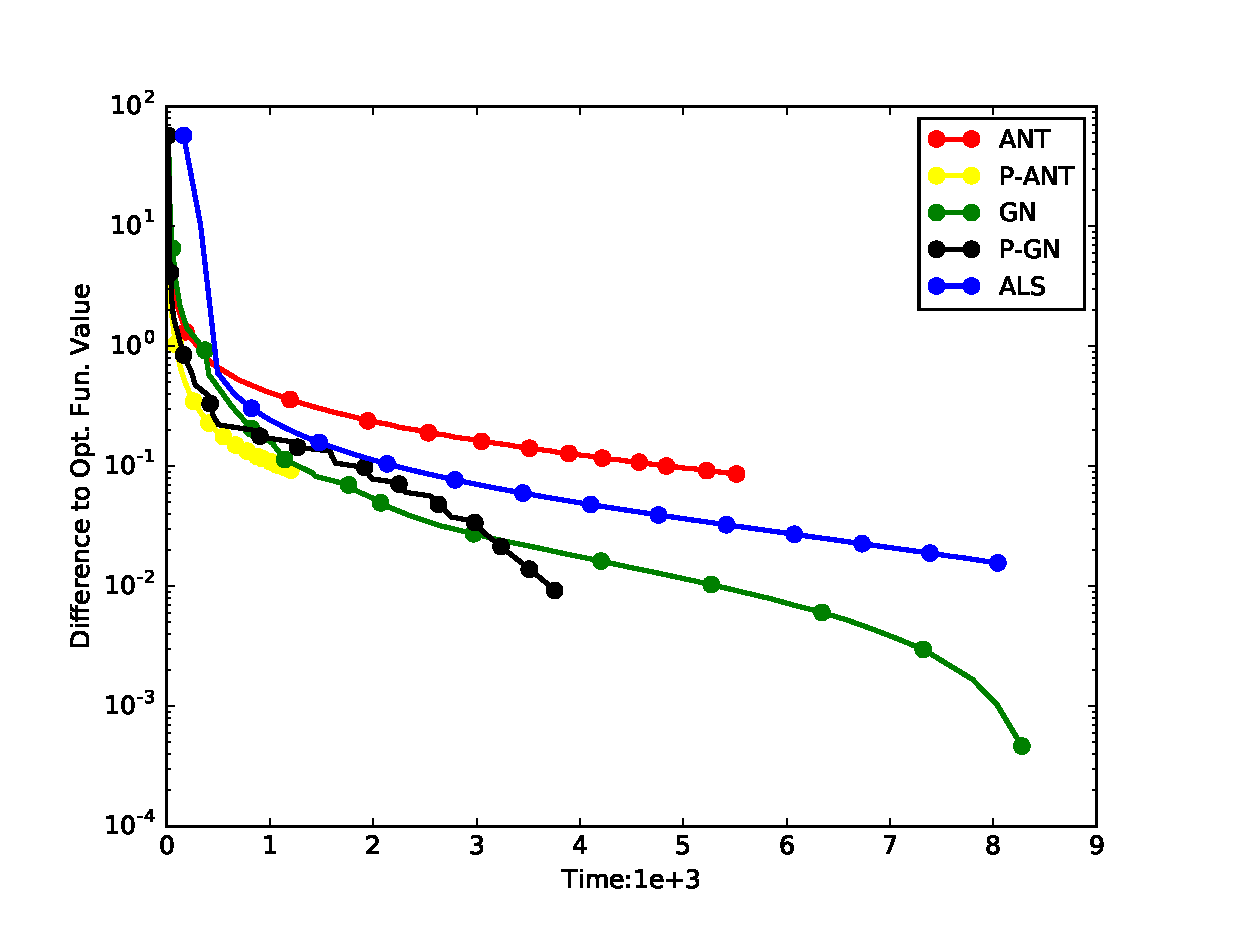
\includegraphics[width=1.03\textwidth]{./figures/ml.1.obj.eps}
        \caption{\tt movielens10m, $\lambda=1$}
    \end{subfigure}
    \begin{subfigure}[b]{0.32\textwidth}
        \centering
        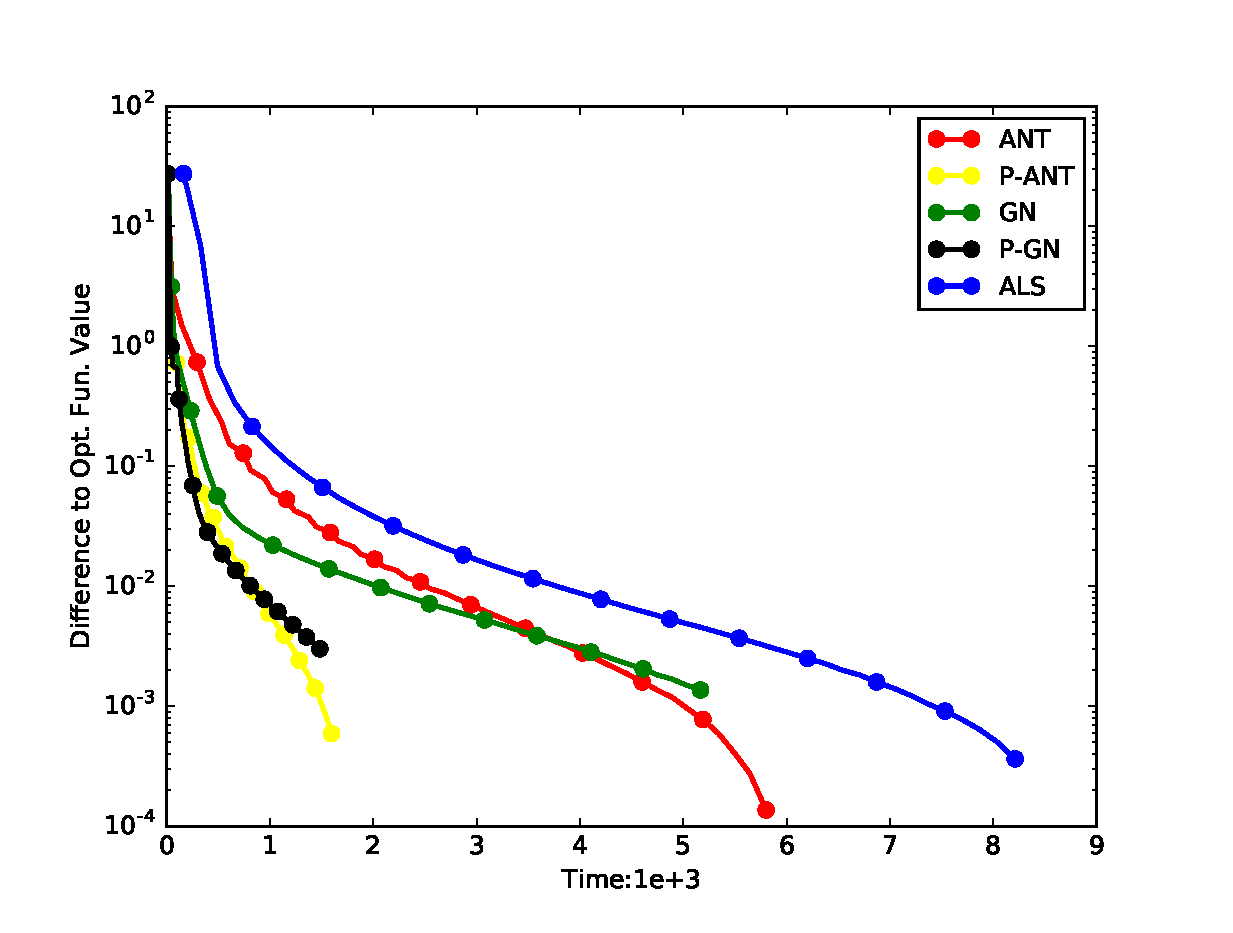
\includegraphics[width=1.03\textwidth]{./figures/ml.8.obj.eps}
        \caption{\tt movielens10m, $\lambda=8$}
    \end{subfigure}
     \begin{subfigure}[b]{0.32\textwidth}
        \centering
        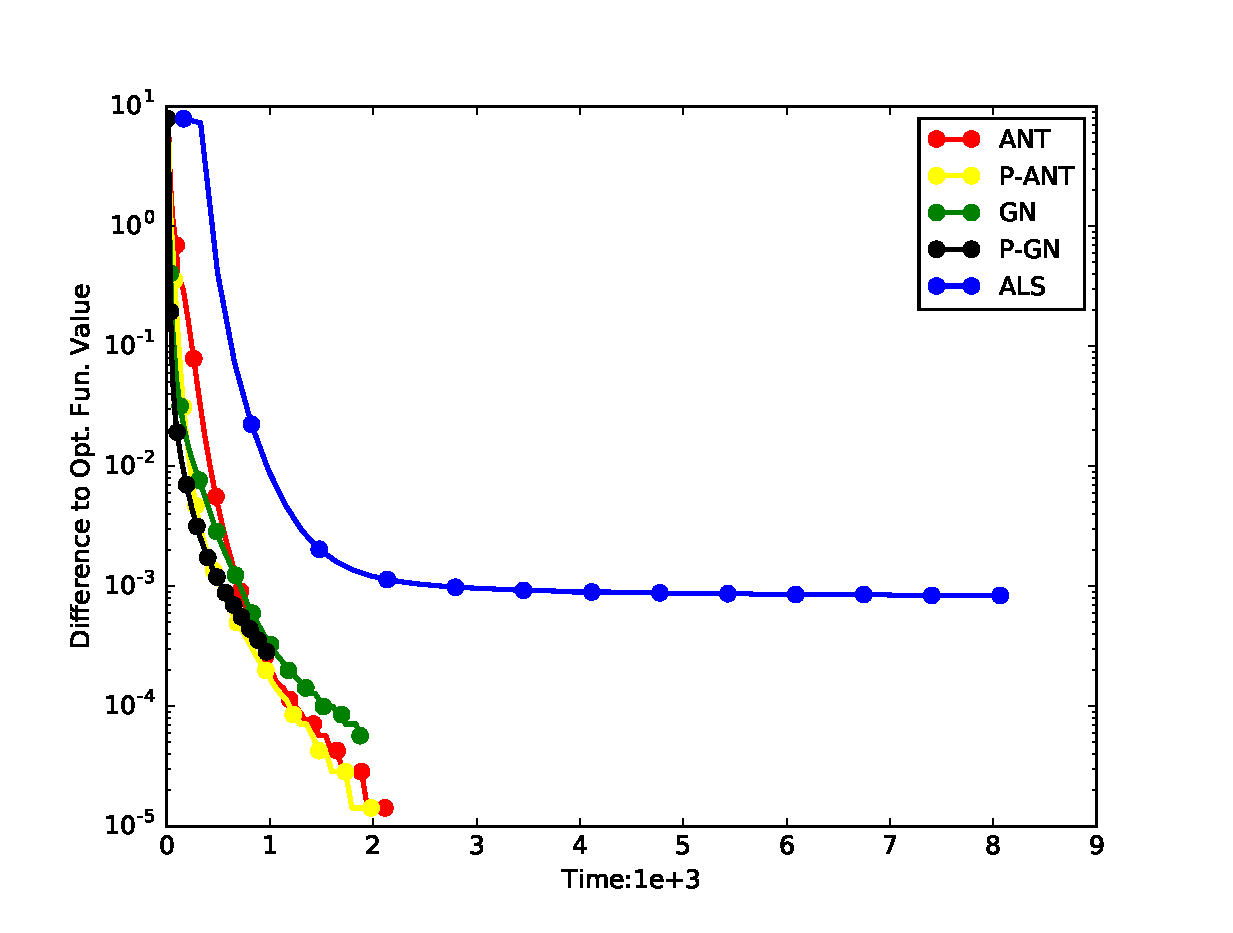
\includegraphics[width=1.03\textwidth]{./figures/ml.64.obj.eps}
        \caption{\tt movielens10m, $\lambda=64$}
    \end{subfigure}
    \begin{subfigure}[b]{0.32\textwidth}
        \centering
        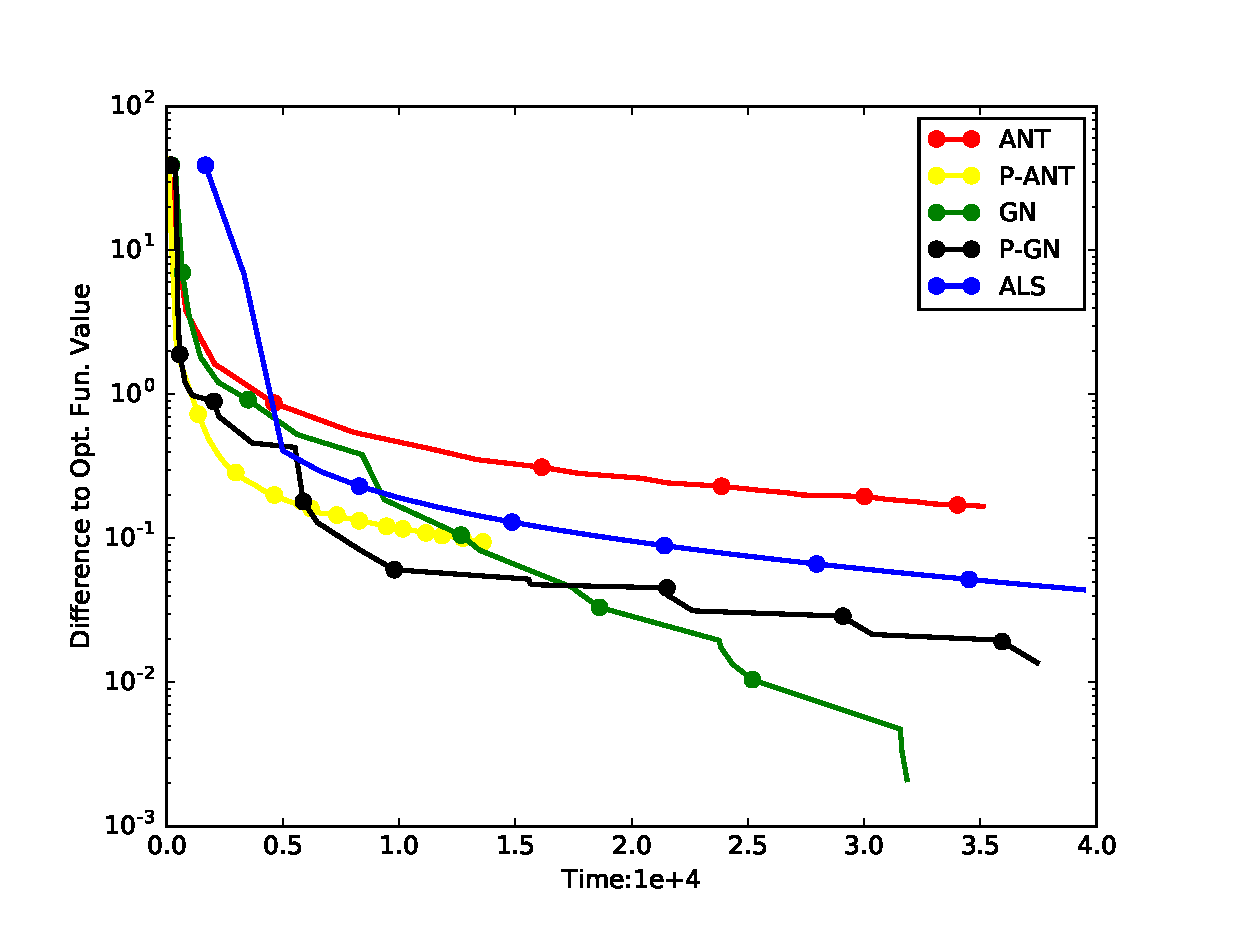
\includegraphics[width=1.03\textwidth]{./figures/nf.1.obj.eps}
        \caption{\tt netflix $\lambda=1$}
    \end{subfigure}
    \begin{subfigure}[b]{0.32\textwidth}
        \centering
        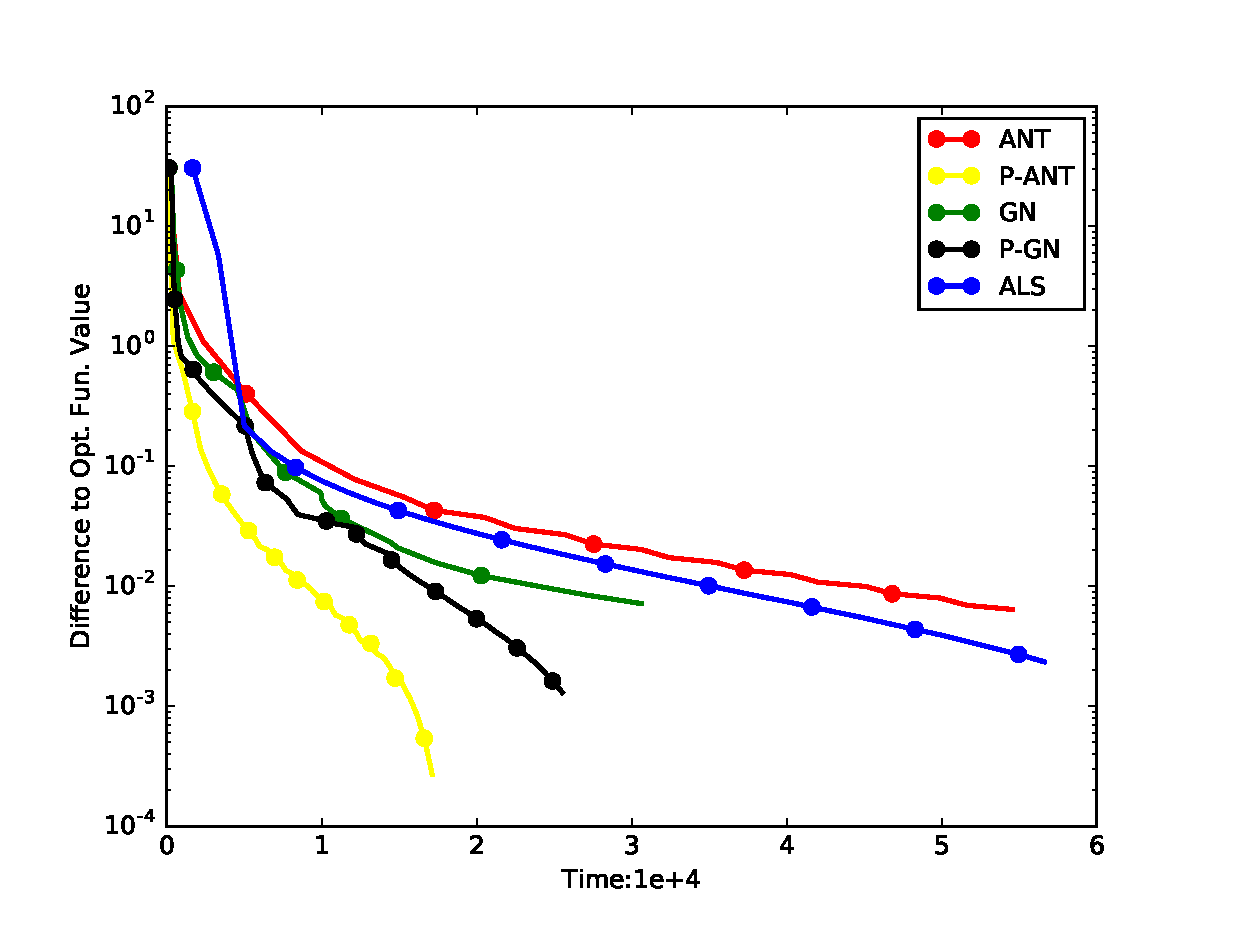
\includegraphics[width=1.03\textwidth]{./figures/nf.8.obj.eps}
        \caption{\tt netflix $\lambda=8$}
    \end{subfigure}
    \begin{subfigure}[b]{0.32\textwidth}
        \centering
        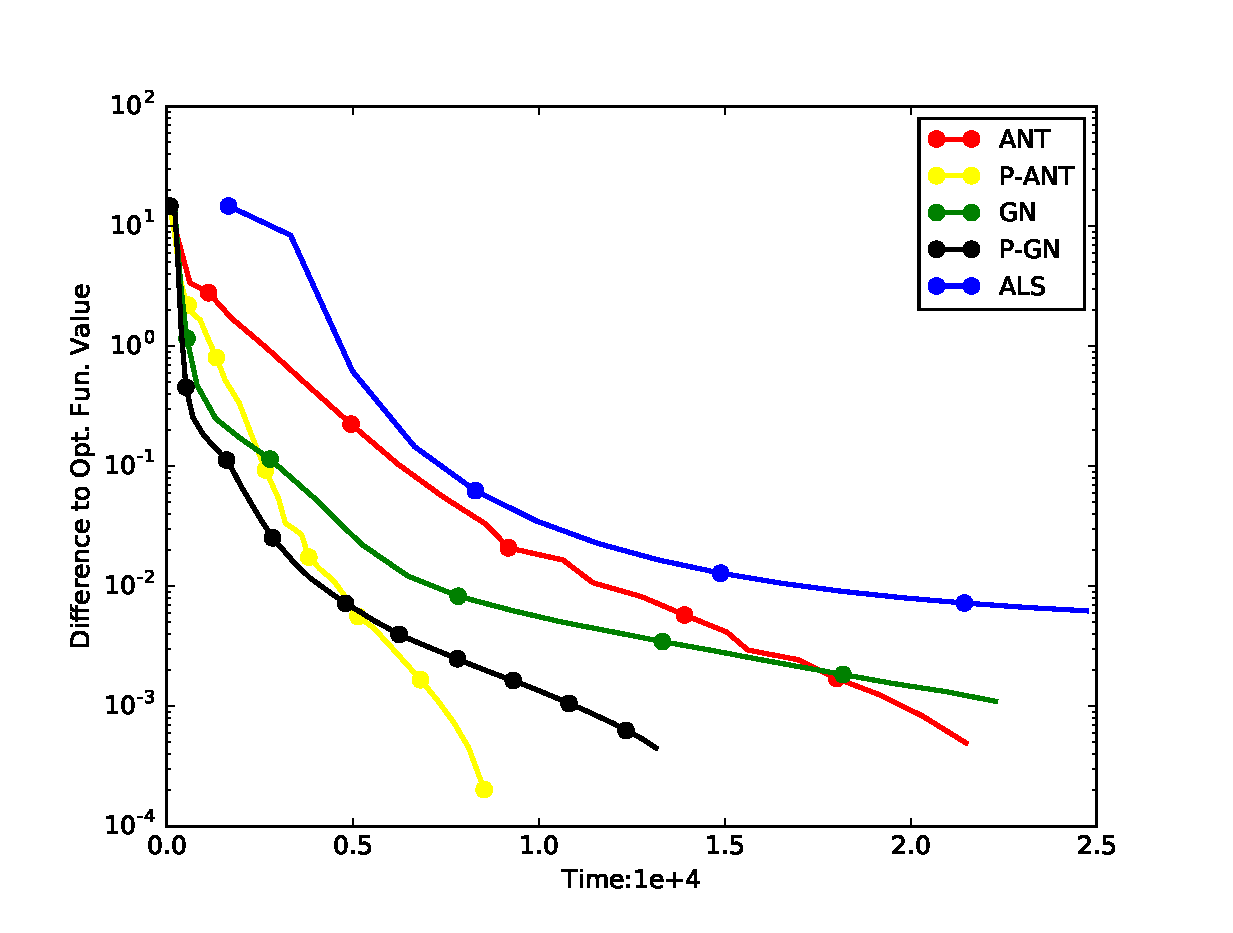
\includegraphics[width=1.03\textwidth]{./figures/nf.64.obj.eps}
        \caption{\tt netflix $\lambda=64$}
    \end{subfigure}
        \caption{Comparison among GN, ALS, ANT, GN-P, ANT-P.
             The $x$-axis is the time which is in seconds.
             The $y$-axis is the log-scaled distance to a local optimal objective value.}
    \label{fig:objvstime}
\end{figure}

\begin{figure}
    \centering
    \begin{subfigure}[b]{0.32\textwidth}
        \centering
        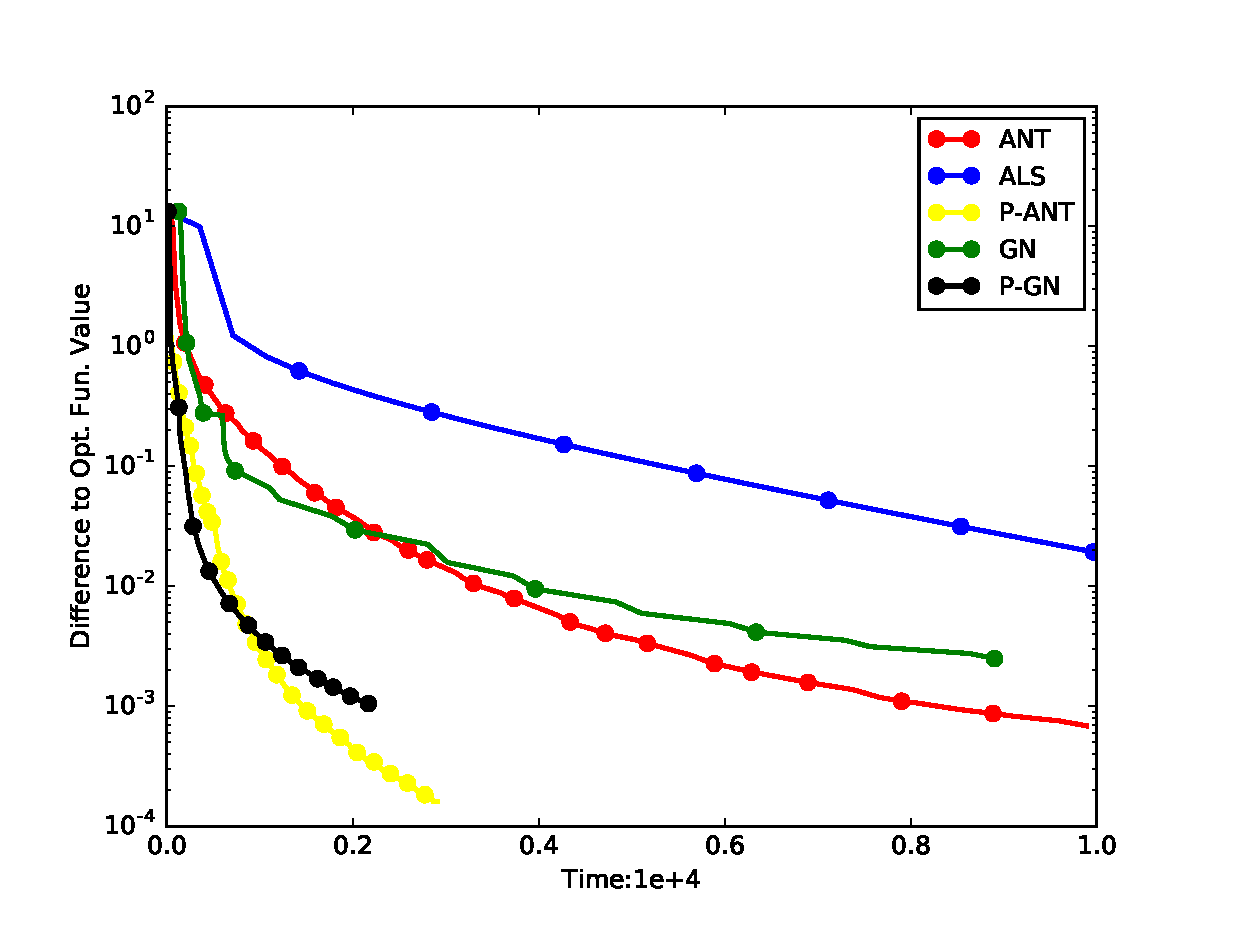
\includegraphics[width=1.03\textwidth]{./figures/ml.obj.eps}
        \caption{\tt movielens10m, $\lambda=0.05$}
    \end{subfigure}
    \begin{subfigure}[b]{0.32\textwidth}
        \centering
        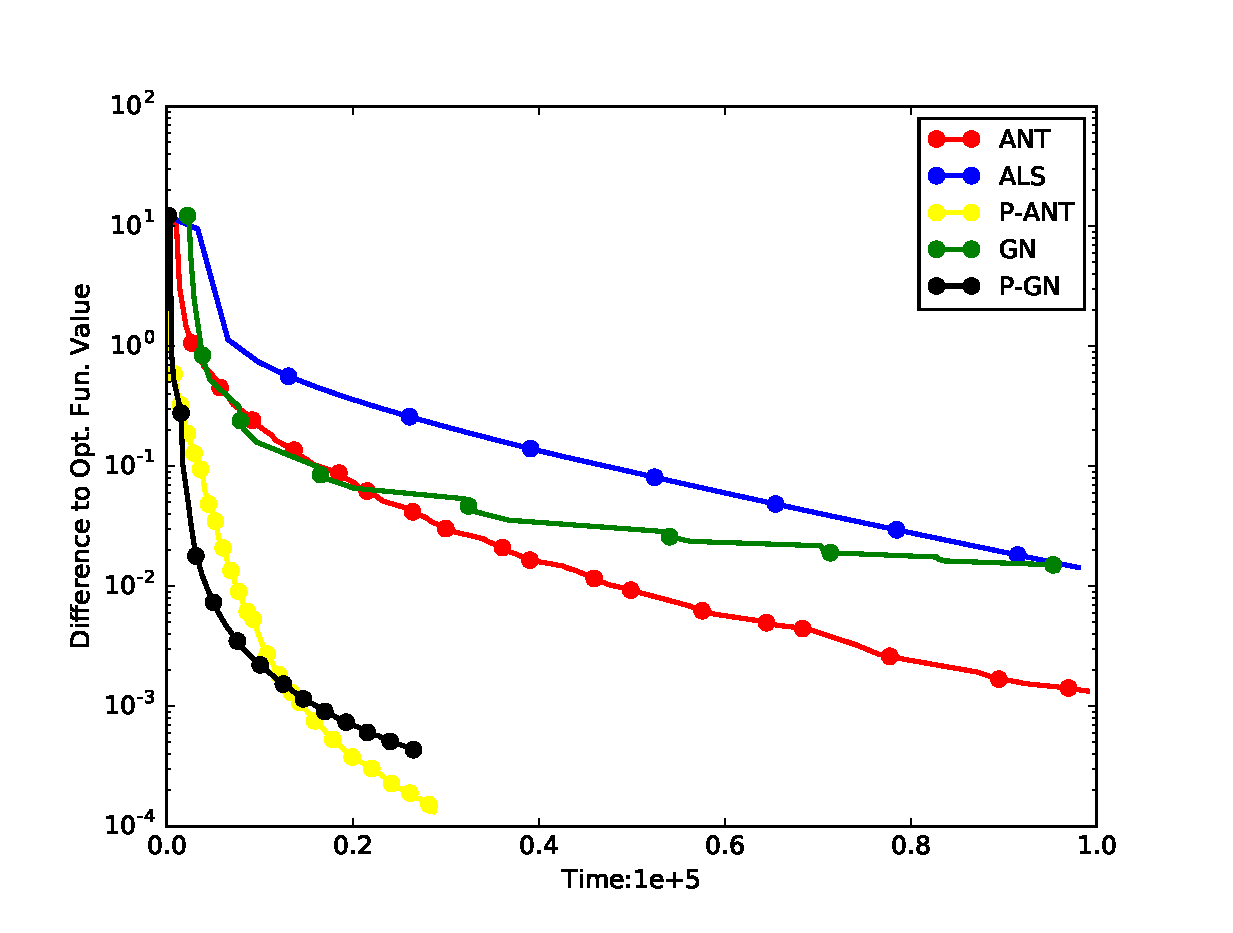
\includegraphics[width=1.03\textwidth]{./figures/nf.obj.eps}
        \caption{\tt netflix, $\lambda=0.05$}
    \end{subfigure}
        \caption{Comparison among GN, ALS, ANT, GN-P, ANT-P.
             The $x$-axis is the time which is in seconds.
             The $y$-axis is the log-scaled distance to a local optimal objective value.}
    \label{fig:freqobjvstime}
\end{figure}

\begin{figure}
    \centering
    \begin{subfigure}[b]{0.32\textwidth}
        \centering
        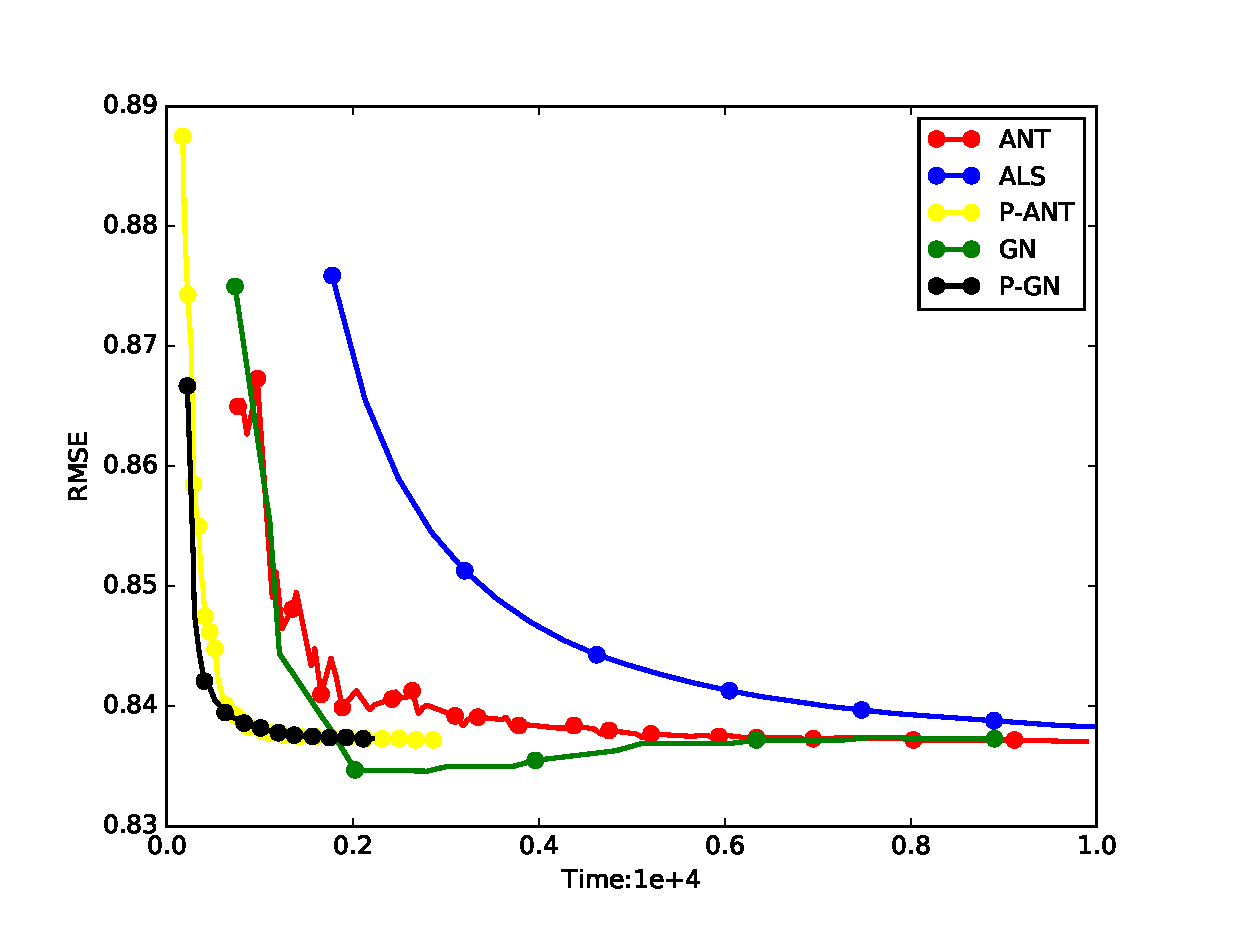
\includegraphics[width=1.03\textwidth]{./figures/ml.rmse.eps}
        \caption{\tt movielens10m, $\lambda=0.05$}
    \end{subfigure}
    \begin{subfigure}[b]{0.32\textwidth}
        \centering
        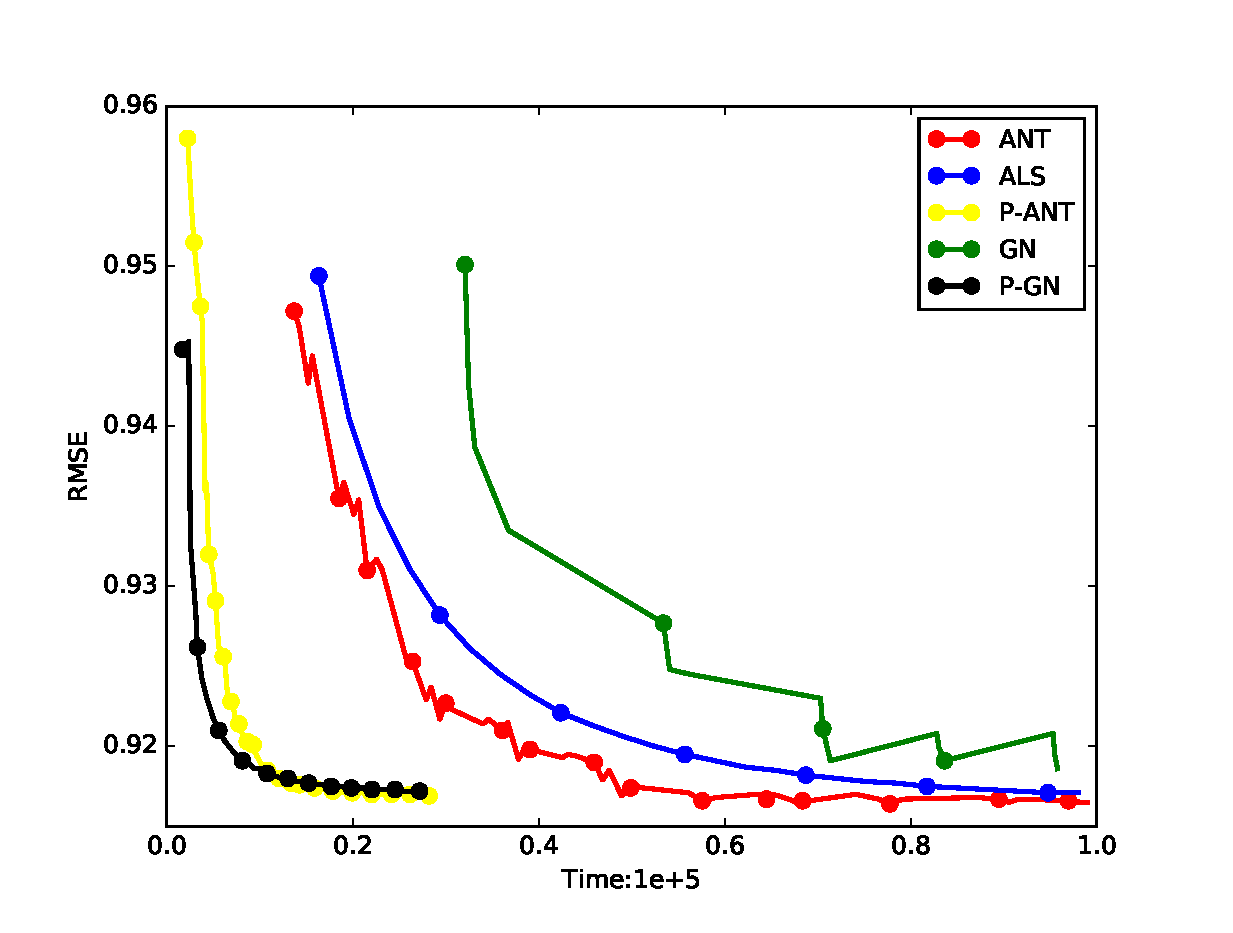
\includegraphics[width=1.03\textwidth]{./figures/nf.rmse.eps}
        \caption{\tt netflix, $\lambda=0.05$}
    \end{subfigure}
        \caption{Comparison among GN, ALS, ANT, GN-P, ANT-P.
             The $x$-axis is the time which is in seconds.
             The $y$-axis is the RMSE.}
    \label{fig:freqrmsevstime}
\end{figure}
\fi

\begin{figure}
	\centering
        \begin{tabular}[t]{ccc}
	
	\setcounter{subfigure}{0}
	\subfloat[\tt movielens10m, $\lambda=1$]{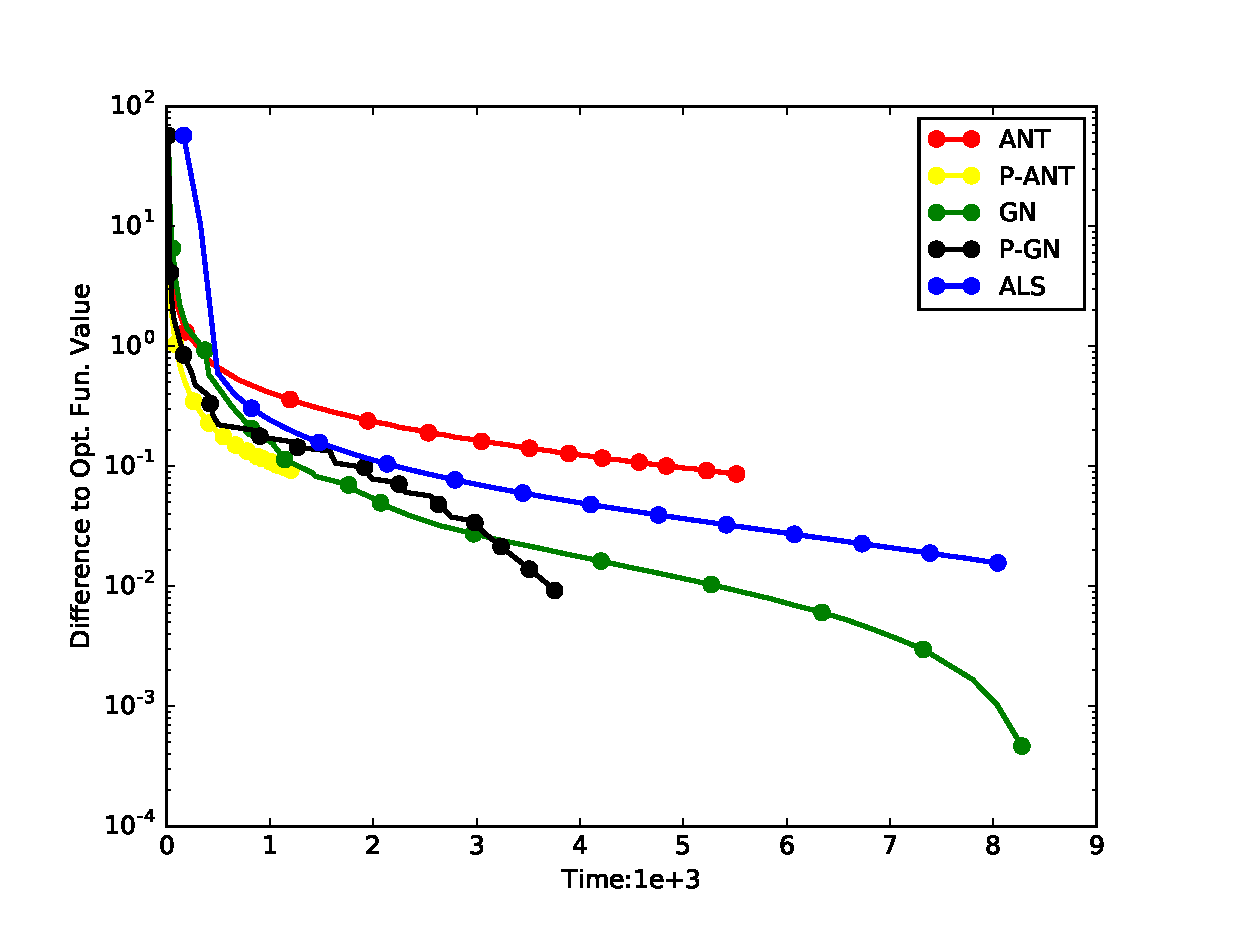
\includegraphics[width=5cm]{./figures/ml.1.obj.eps}}
	&
	\subfloat[\tt movielens10m, $\lambda=8$]{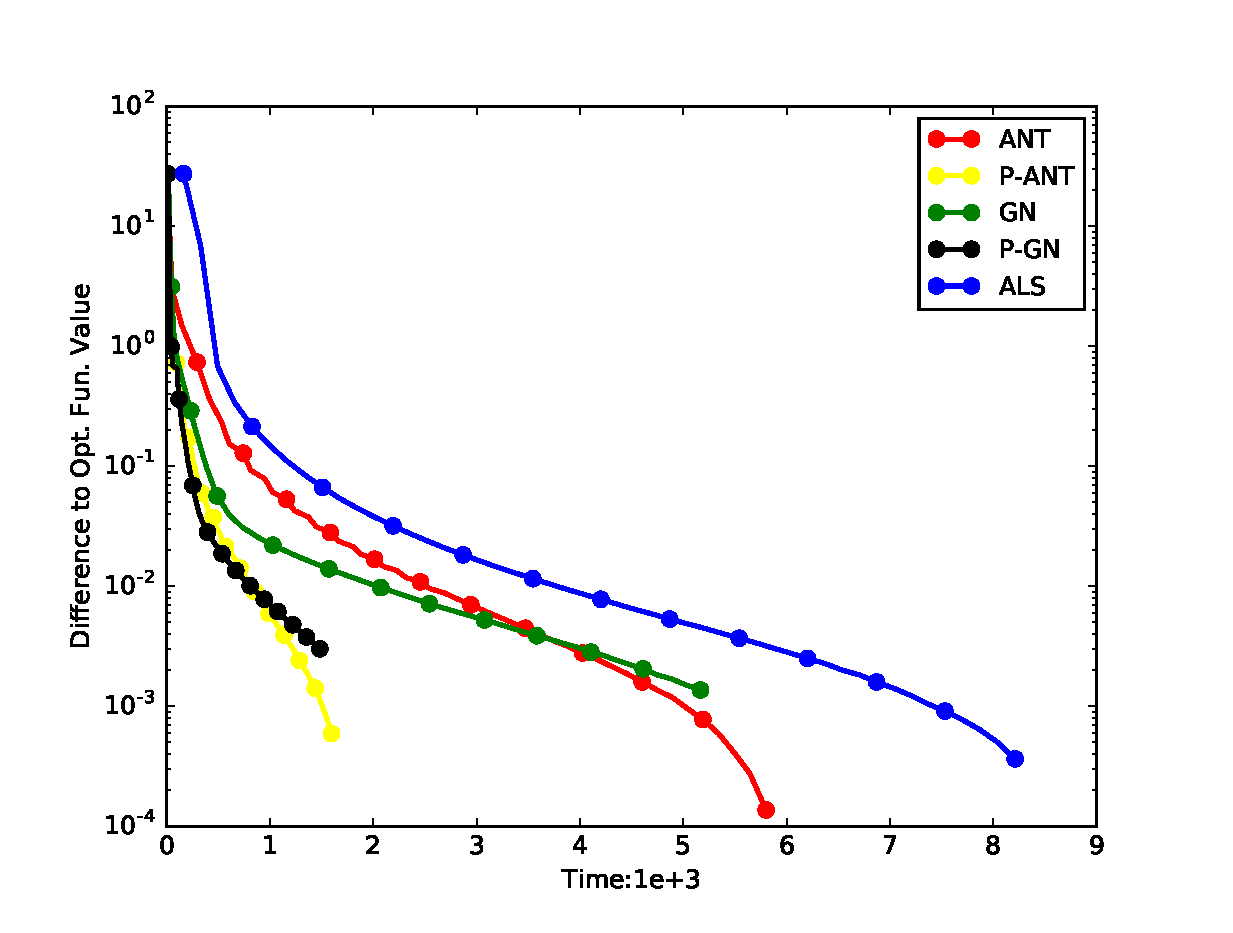
\includegraphics[width=5cm]{./figures/ml.8.obj.eps}}
	&
	\subfloat[\tt movielens10m, $\lambda=64$]{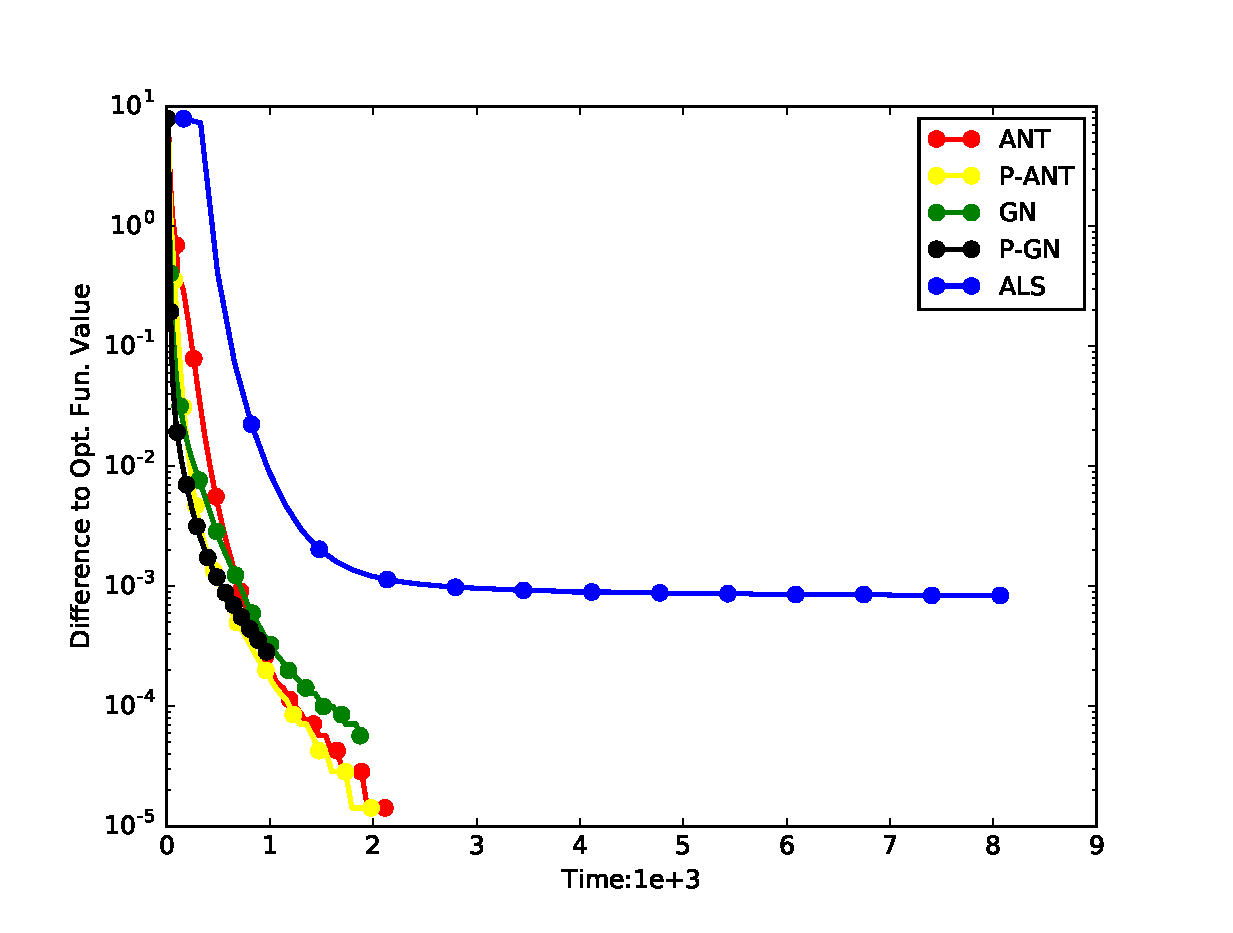
\includegraphics[width=5cm]{./figures/ml.64.obj.eps}}
	
	\\
	\setcounter{subfigure}{3}
	\subfloat[\tt netflix, $\lambda=1$]{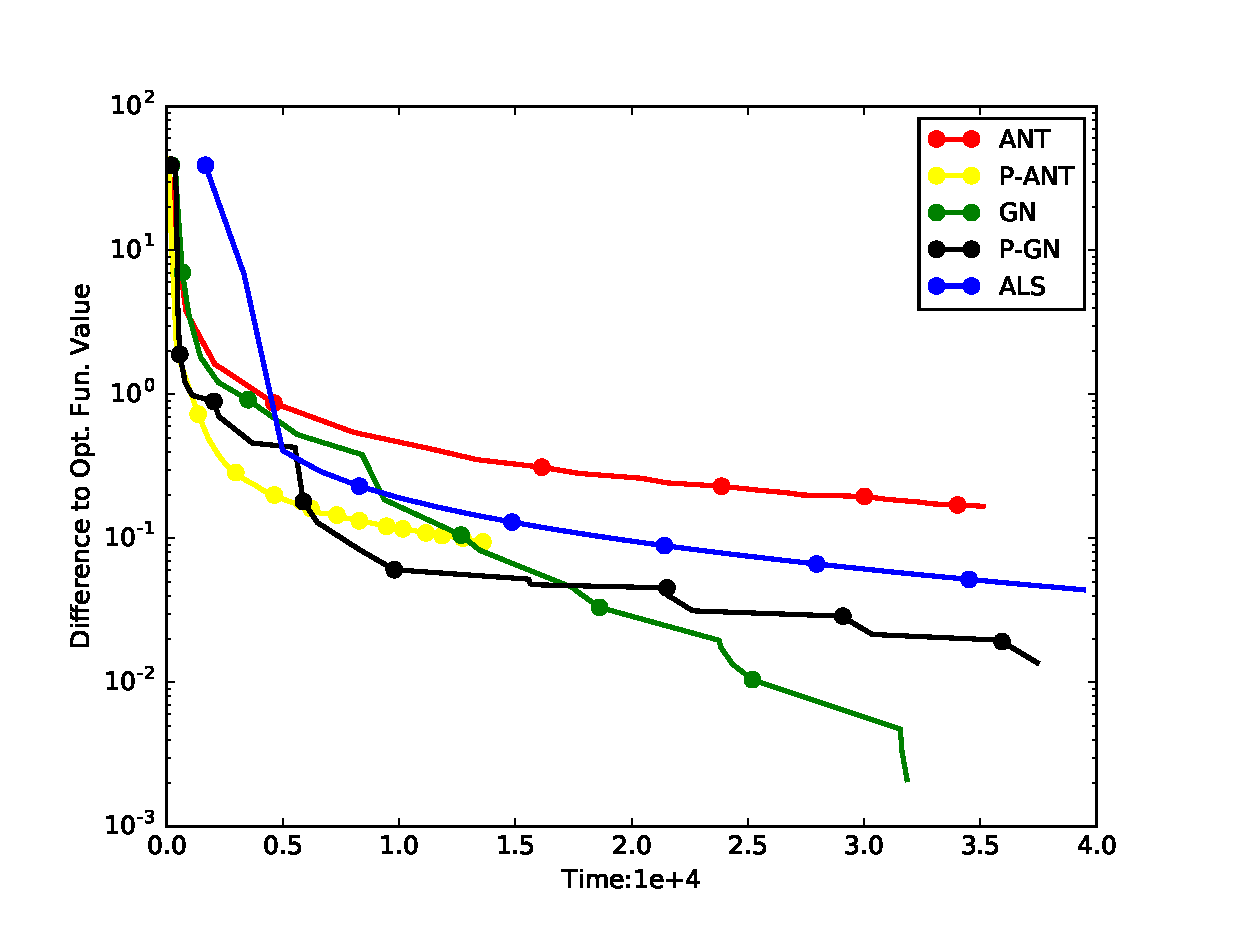
\includegraphics[width=5cm]{./figures/nf.1.obj.eps}}
	&
	\subfloat[\tt netflix, $\lambda=8$]{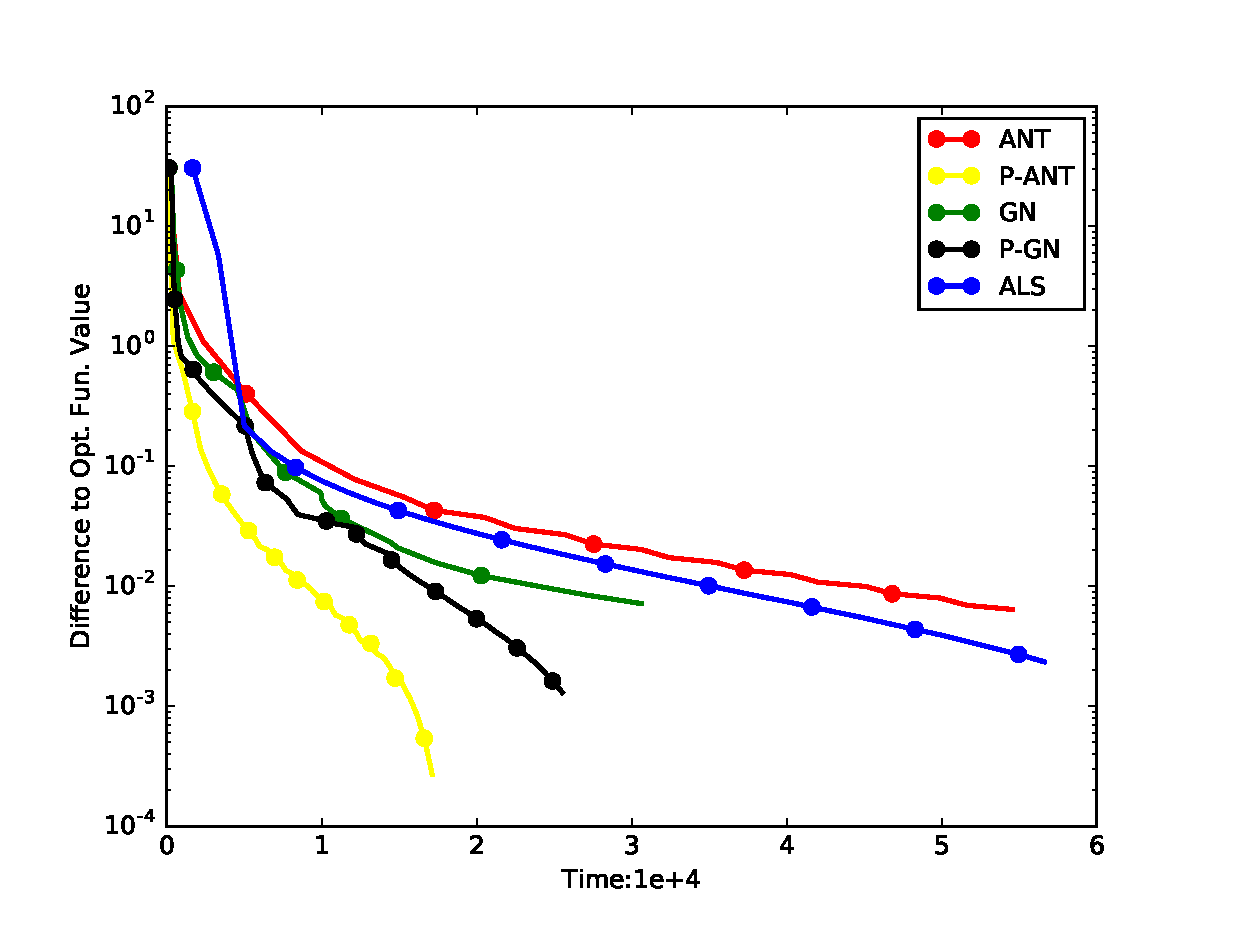
\includegraphics[width=5cm]{./figures/nf.8.obj.eps}}
	&
	\subfloat[\tt netflix, $\lambda=64$]{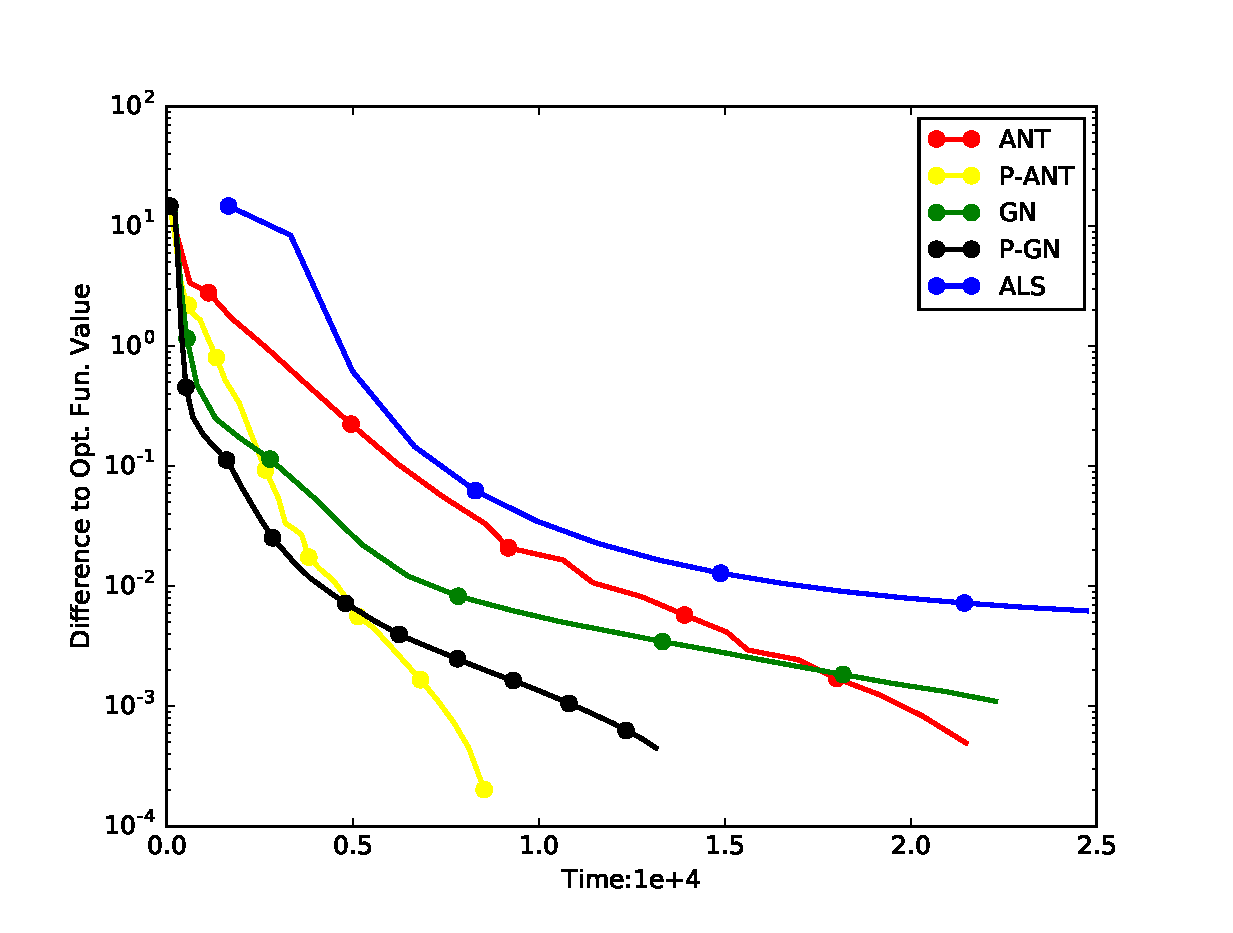
\includegraphics[width=5cm]{./figures/nf.64.obj.eps}}
	\end{tabular}
	\caption{Comparison among GN, ALS, ANT, GN-P, ANT-P.
             The $x$-axis is the time which is in seconds.
             The $y$-axis is the log-scaled distance to a local optimal objective value.} \label{fig:objvstime}
\end{figure}

\begin{figure}
	\centering
        \begin{tabular}[t]{cc}
	
	\setcounter{subfigure}{0}
	\subfloat[\tt movielens10m, $\lambda=0.05$]{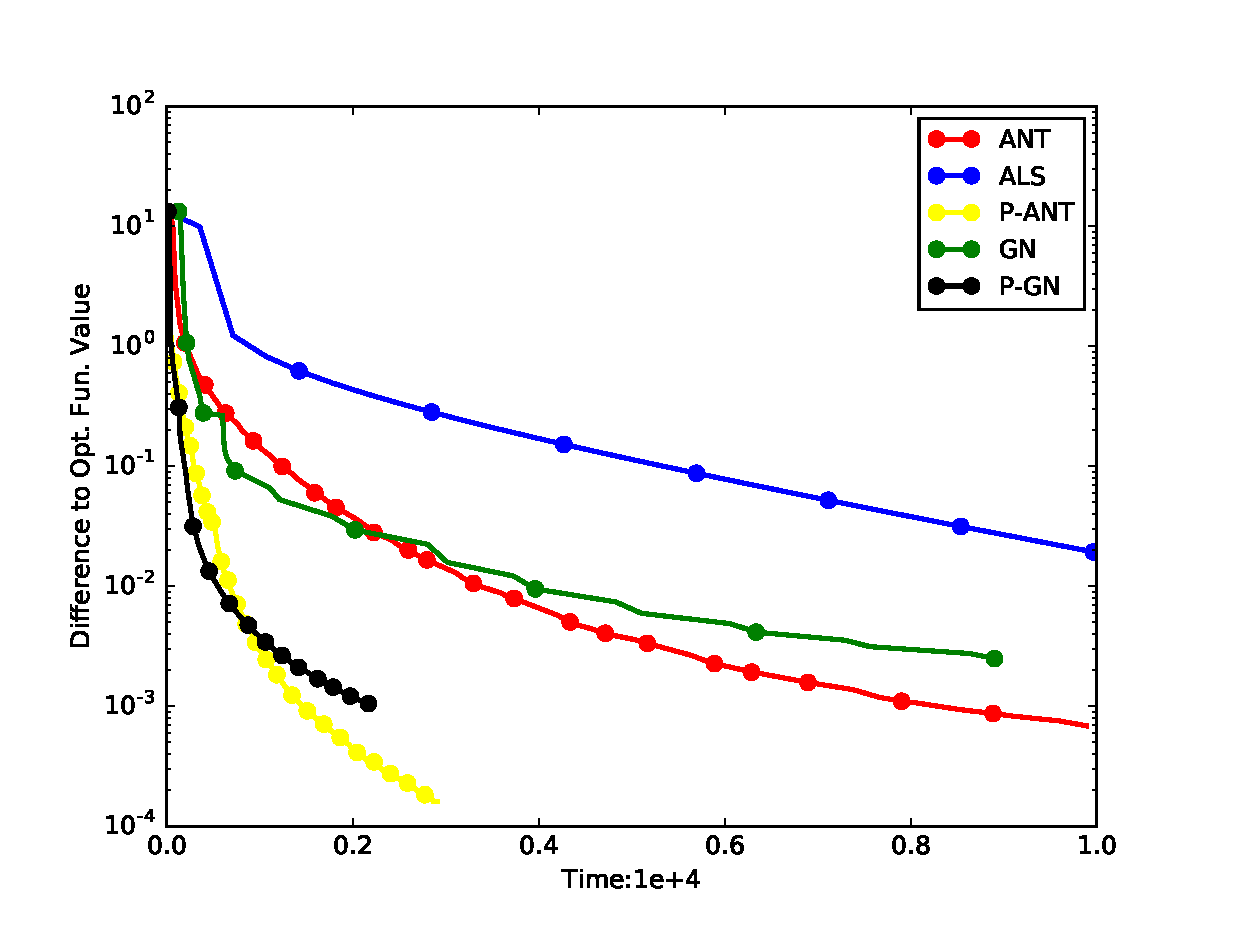
\includegraphics[width=7cm]{./figures/ml.obj.eps}}
	&
	\subfloat[\tt netflix, $\lambda=0.05$]{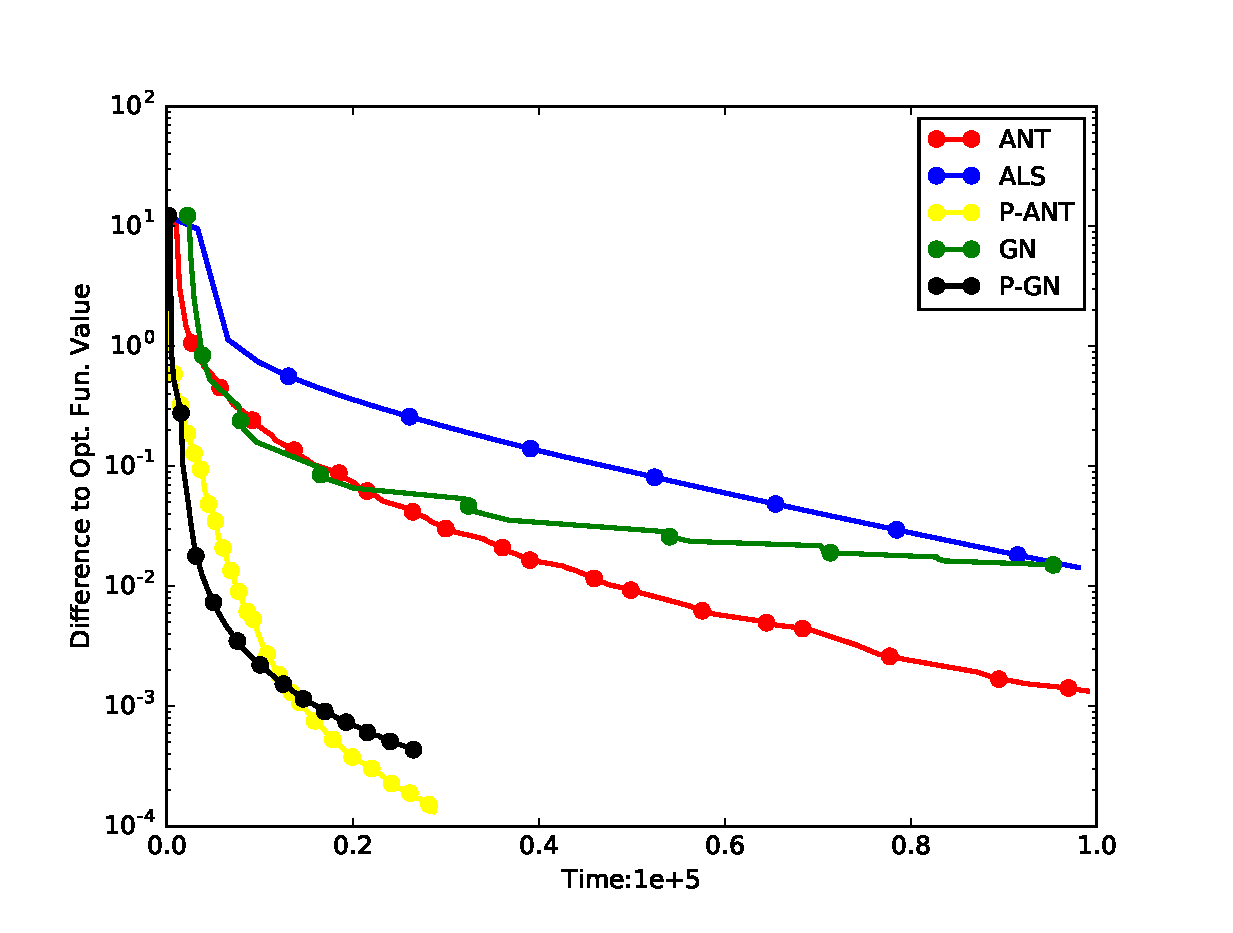
\includegraphics[width=7cm]{./figures/nf.obj.eps}}

	\end{tabular}
	\caption{Comparison among GN, ALS, ANT, GN-P, ANT-P.
             The $x$-axis is the time which is in seconds.
             The $y$-axis is the log-scaled distance to a local optimal objective value.} \label{fig:freqobjvstime}
\end{figure}

\begin{figure}
	\centering
        \begin{tabular}[t]{cc}
	
	\setcounter{subfigure}{0}
	\subfloat[\tt movielens10m, $\lambda=0.05$]{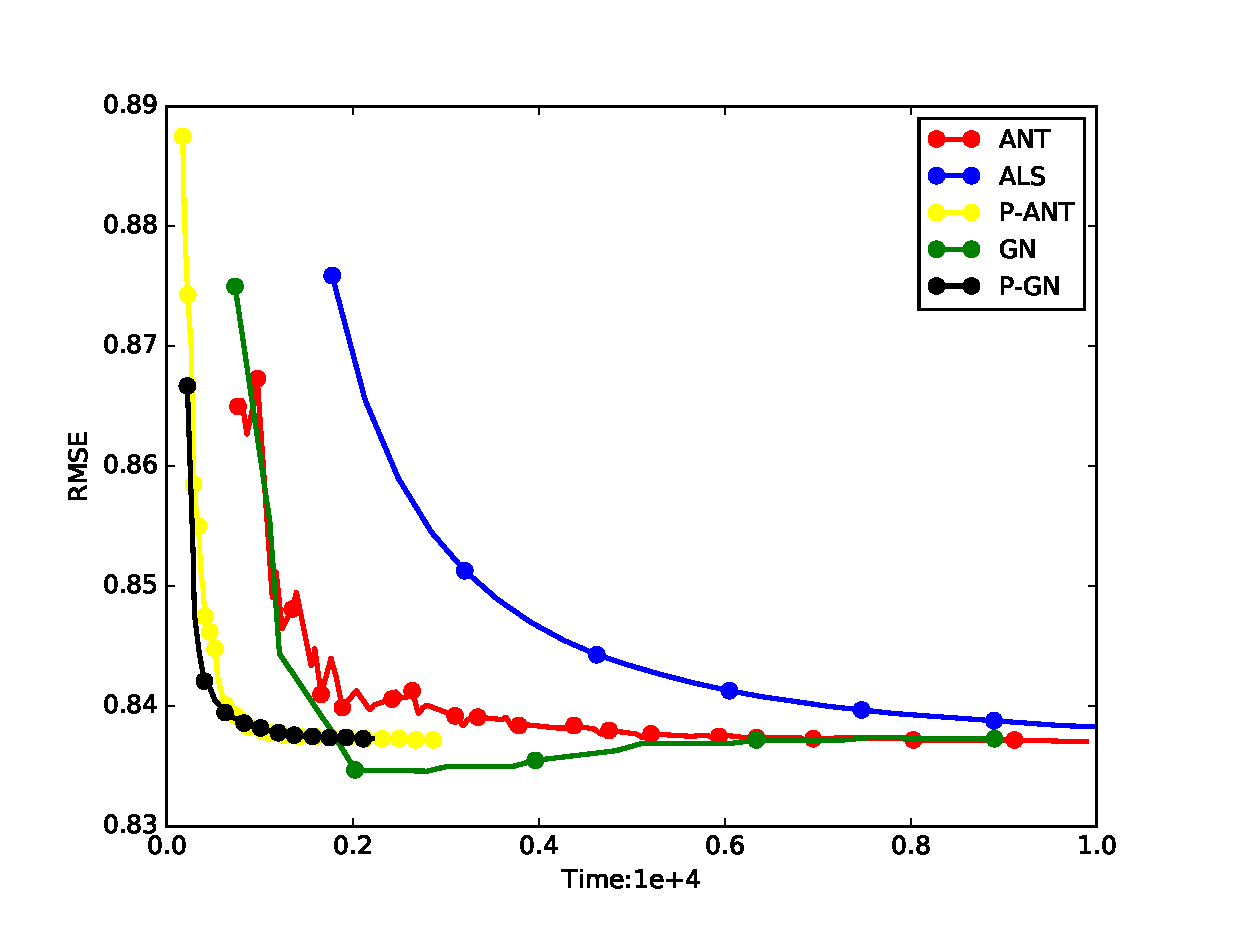
\includegraphics[width=7cm]{./figures/ml.rmse.eps}}
	&
	\subfloat[\tt netflix, $\lambda=0.05$]{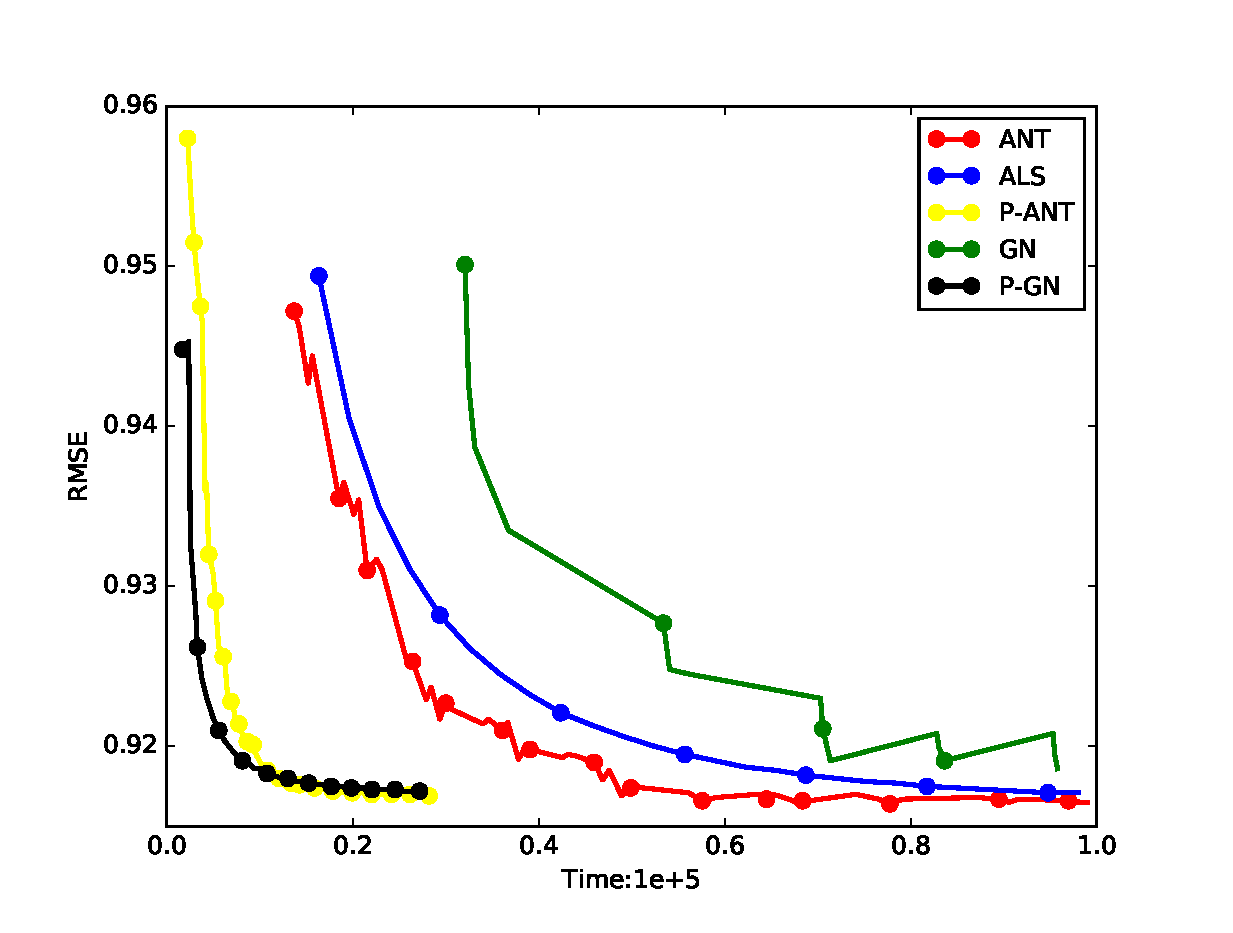
\includegraphics[width=7cm]{./figures/nf.rmse.eps}}
	
	
	\end{tabular}
	\caption{Comparison among GN, ALS, ANT, GN-P, ANT-P.
             The $x$-axis is the time which is in seconds.
             The $y$-axis is the RMSE.} \label{fig:freqrmsevstime}
\end{figure}





\clearpage\newpage
%\bibliographystyle{abbrv}
%\bibliography{sdp}


\section{Reproduction of bad cases in ANT and ANT-P}

\begin{table}[H]
\centering
\begin{tabular}{|c|c|c|c|c|c|c|c|c|l|}
\hline
\multicolumn{3}{|c|}{\tt movielens10m}                    & \multicolumn{3}{c|}{\tt neflix}                           & split 1                 & split 2                 & \multicolumn{2}{c|}{split 3}                 \\ \hline
\multirow{2}{*}{rating} & \multicolumn{2}{c|}{number} & \multirow{2}{*}{rating} & \multicolumn{2}{c|}{number} & \multirow{2}{*}{rating} & \multirow{2}{*}{rating} & \multicolumn{2}{c|}{\multirow{2}{*}{rating}} \\ \cline{2-3} \cline{5-6}
                        & tr            & va(te)          &                         & tr            & va(te)          &                         &                         & \multicolumn{2}{c|}{}                        \\ \hline
0.5$\sim$2              & 1300280       & 87454       & 1                       & 4544779       & 73211       & 1                       & 1                       & \multicolumn{2}{c|}{1}                       \\ \hline
2.5$\sim$5              & 8000994       & 611308      & 2$\sim$5                & 94527333      & 1335184     & 5                       & 50                      & \multicolumn{2}{c|}{100}                     \\ \hline
\end{tabular}
\caption{Distributions of ratings.}
\label{tab:dist}
\end{table}

We try to reproduce bad cases in ANT and ANT-P and then compare how the performance of GN and GN-P is in the situation, so we rebuild imbalance datas from {\tt movielens10m} and {\tt netflix}. There are 1300280 instances those ratings which are less than or equal to 2 and 8000994 instances those ratings which are larger than 2 in training data of {\tt movielens10m} in total. In order to build imbalance data, we change those ratings which are less than or equal to 2 to 1 and change the other ratings to 5 (split 1), 50 (split 2) or 100 (split 3) from original {\tt movielens10m} data. Similarly there are 4544779 instances those ratings which are equal to 1 and 94527333 instances those ratings which are larger than 1 in training data of {\tt netflix}, and we change those ratings which are large than 1 to 5 (split 1), 50 (split 2) or 100 (split 3). The distribution of ratings of these imbalance data shows in Table \ref{tab:dist}.
%The results are shown in Table \ref{tab:RMSEMovieLens}-\ref{tab:RMSENetflix}.


{\setlength{\textfloatsep}{0pt}
\begin{figure}[h!]
	\centering
        \begin{tabular}[t]{ccc}
	\subfloat{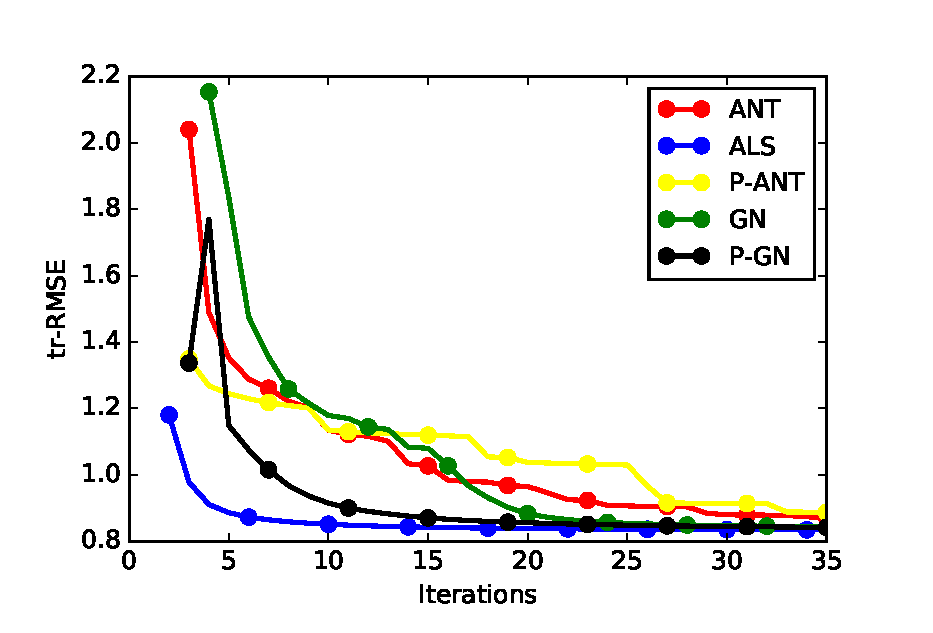
\includegraphics[width=5cm]{./ctr-like_figures/ml.5.tr-rmse.iter.eps}}
	&
	\subfloat{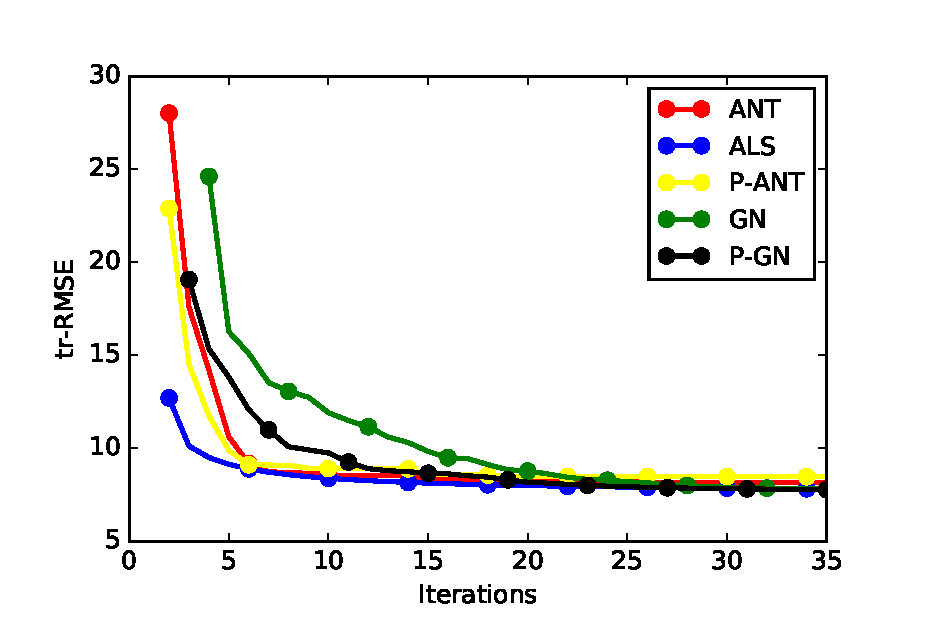
\includegraphics[width=5cm]{./ctr-like_figures/ml.50.tr-rmse.iter.eps}}
	&
	\subfloat{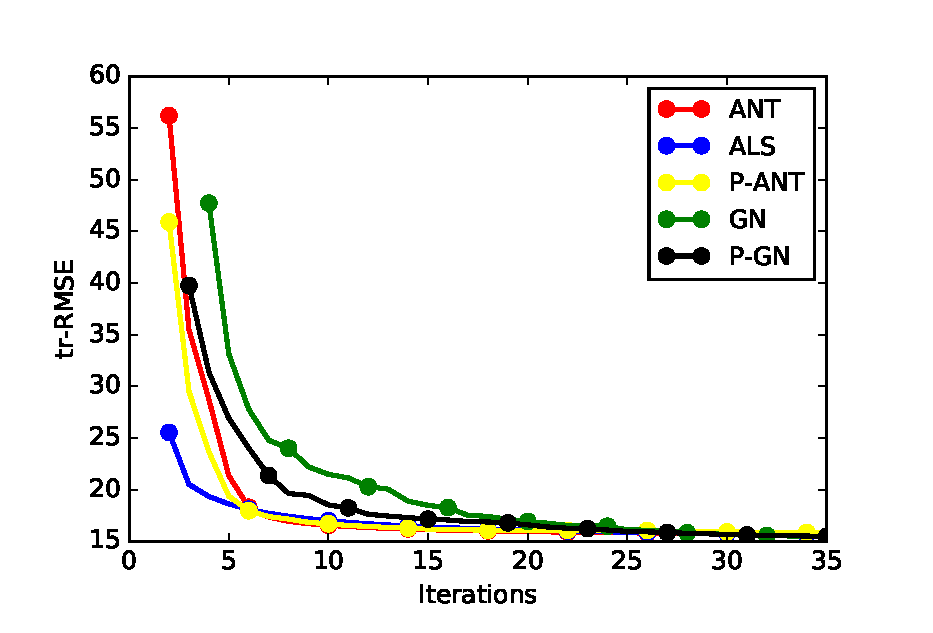
\includegraphics[width=5cm]{./ctr-like_figures/ml.100.tr-rmse.iter.eps}}
	\\
	\setcounter{subfigure}{0}
	\subfloat[\tt movielens10m, split 1]{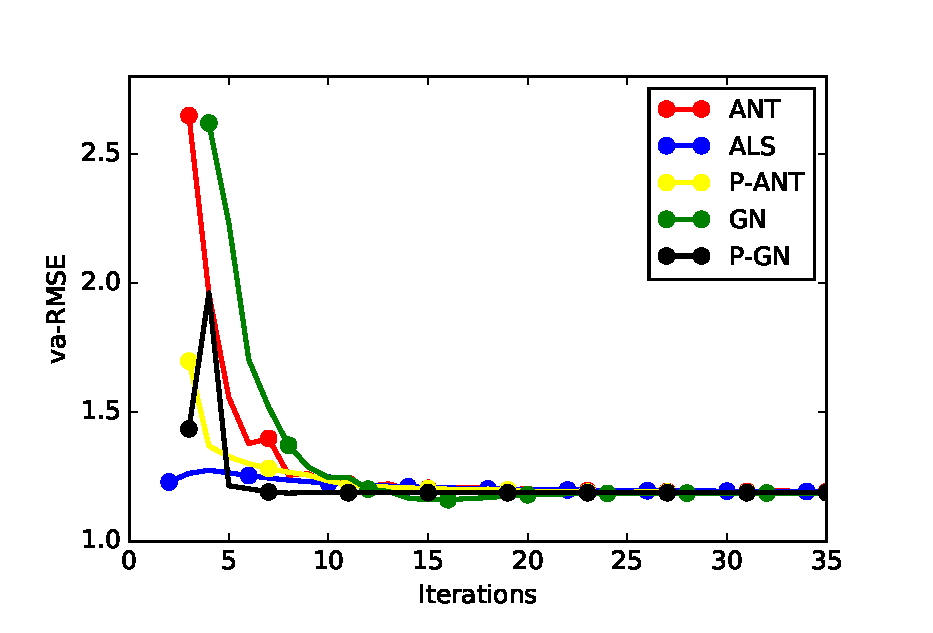
\includegraphics[width=5cm]{./ctr-like_figures/ml.5.va-rmse.iter.eps}}
	&
	\subfloat[\tt movielens10m, split 2]{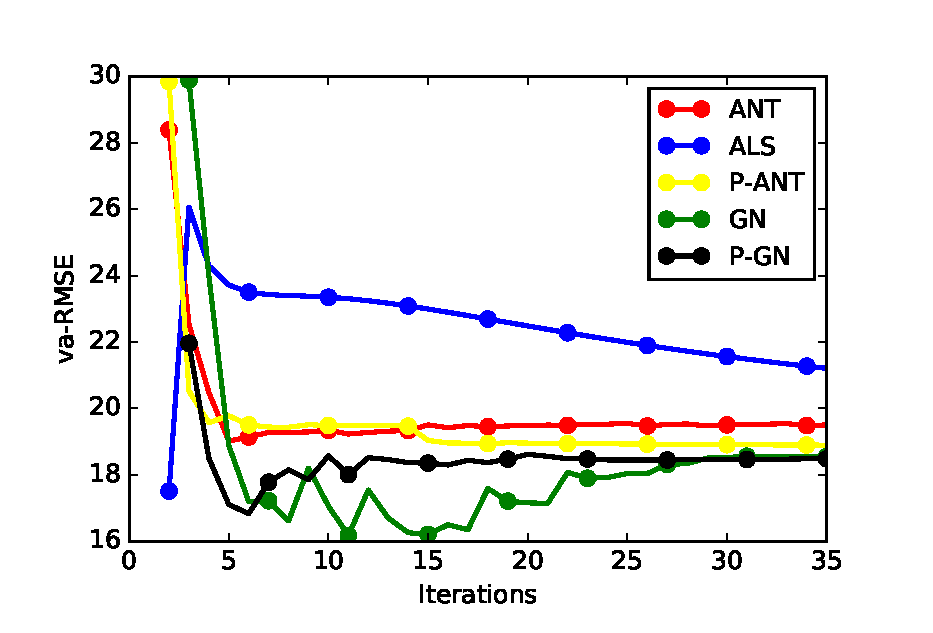
\includegraphics[width=5cm]{./ctr-like_figures/ml.50.va-rmse.iter.eps}}
	&
	\subfloat[\tt movielens10m, split 3]{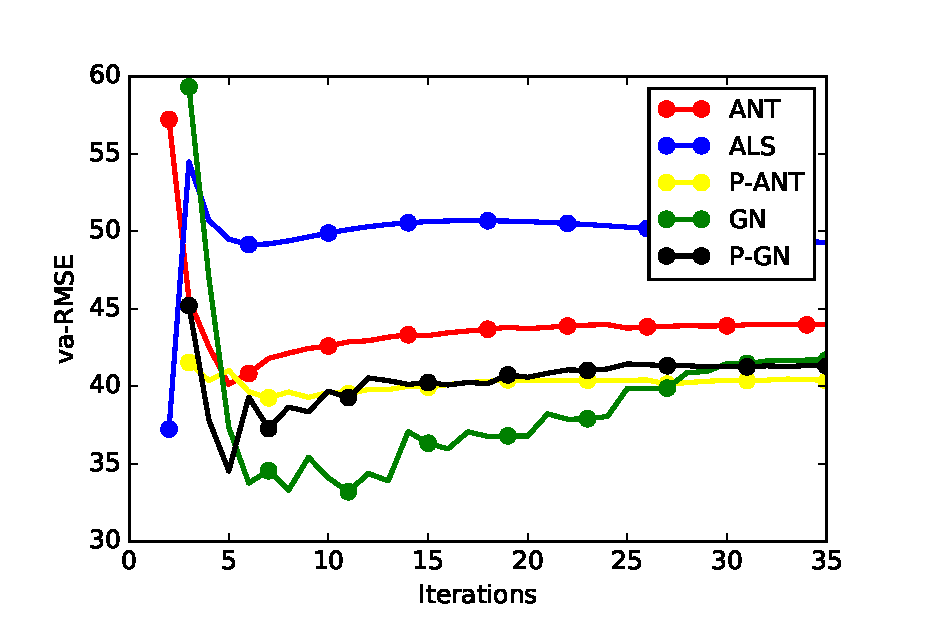
\includegraphics[width=5cm]{./ctr-like_figures/ml.100.va-rmse.iter.eps}}
	\\
	\subfloat{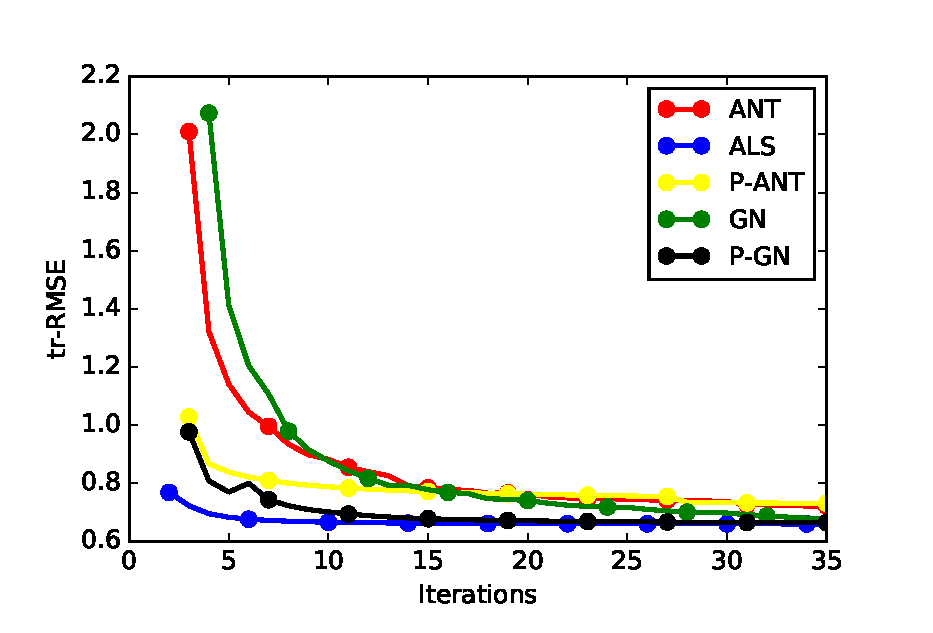
\includegraphics[width=5cm]{./ctr-like_figures/nf.5.tr-rmse.iter.eps}}
	&
	\subfloat{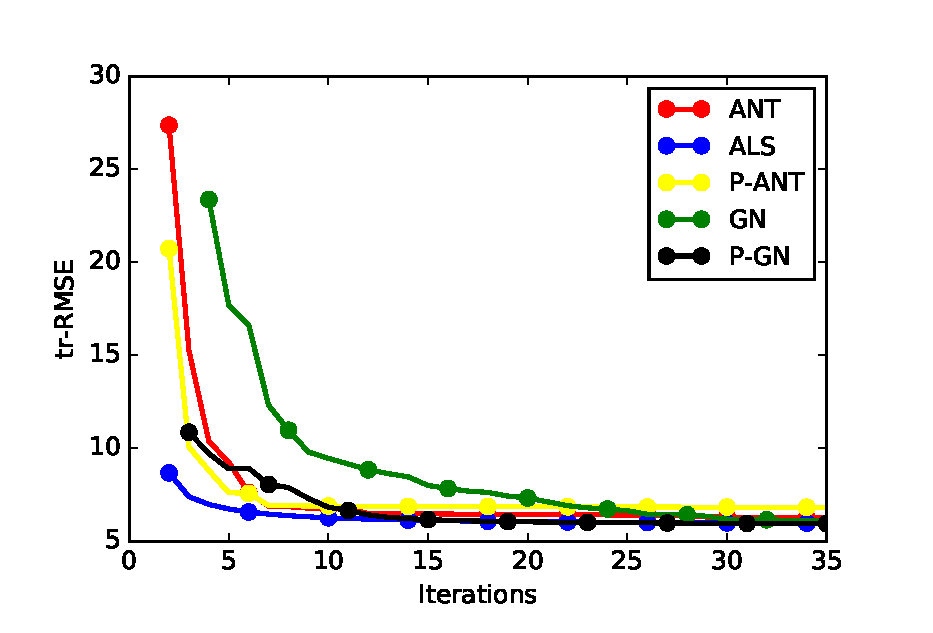
\includegraphics[width=5cm]{./ctr-like_figures/nf.50.tr-rmse.iter.eps}}
	&
	\subfloat{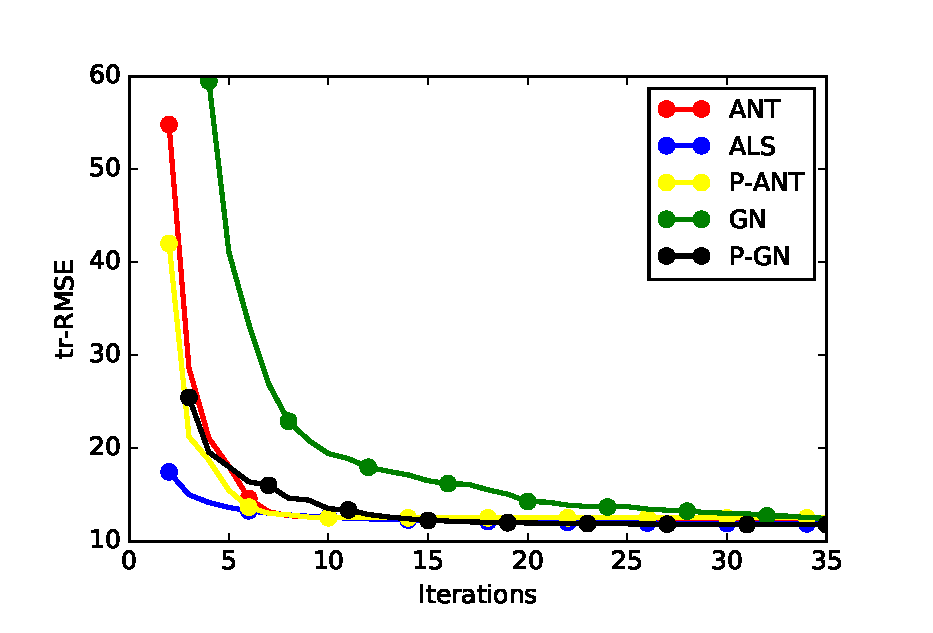
\includegraphics[width=5cm]{./ctr-like_figures/nf.100.tr-rmse.iter.eps}}
	\\
	\setcounter{subfigure}{3}
	\subfloat[\tt netflix, split 1]{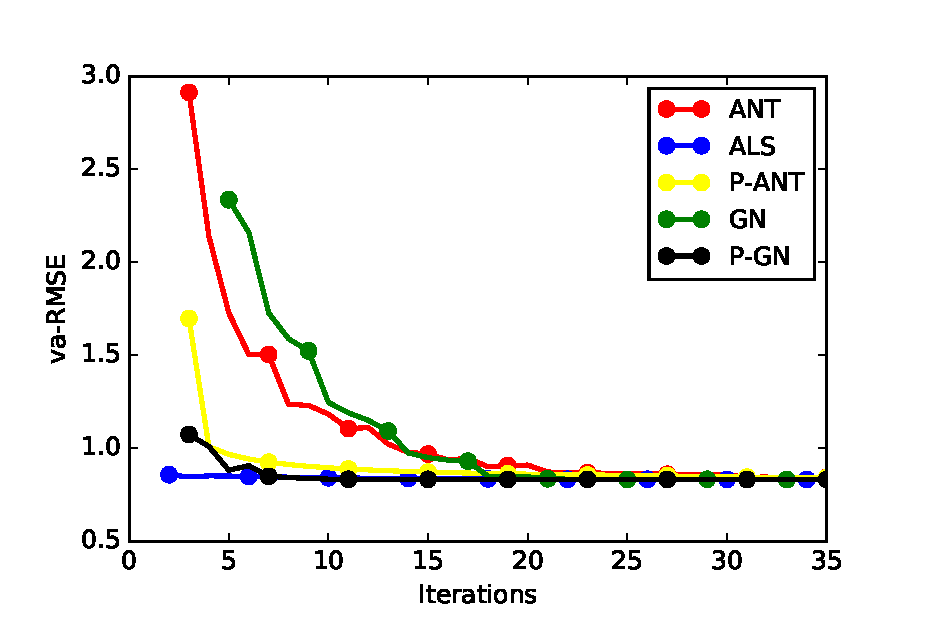
\includegraphics[width=5cm]{./ctr-like_figures/nf.5.va-rmse.iter.eps}}
	&
	\subfloat[\tt netflix, split 2]{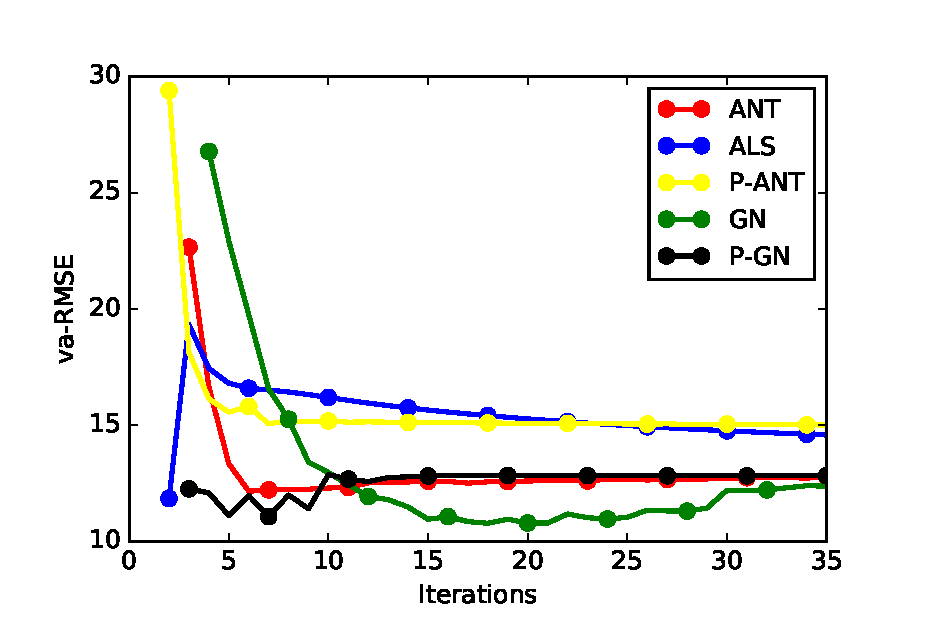
\includegraphics[width=5cm]{./ctr-like_figures/nf.50.va-rmse.iter.eps}}
	&
	\subfloat[\tt netflix, split 3]{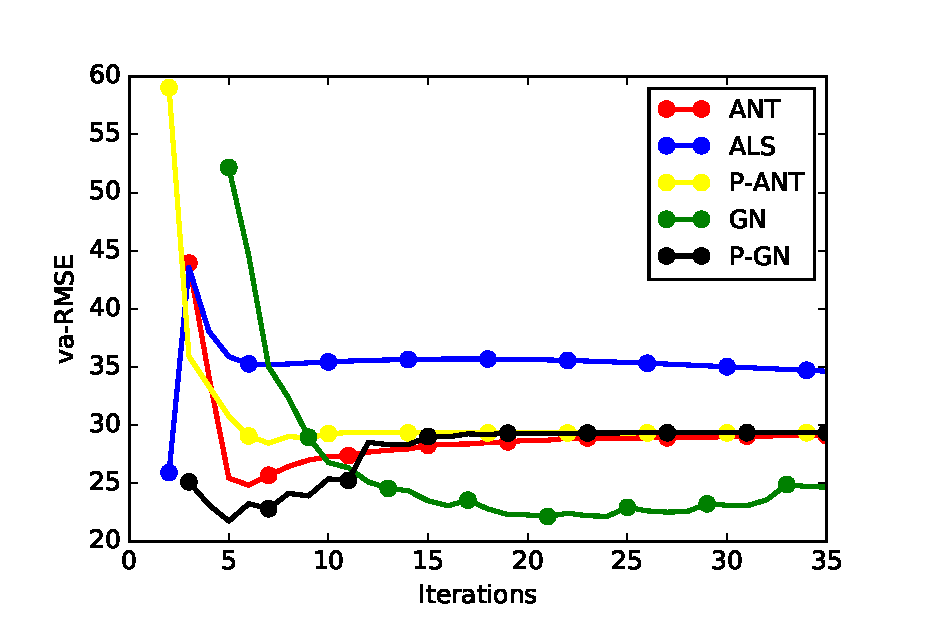
\includegraphics[width=5cm]{./ctr-like_figures/nf.100.va-rmse.iter.eps}}
	\end{tabular}
	\caption{Comparison among GN, ALS, ANT, GN-P, ANT-P. The $x$-axis is the number of outer iteration, For each set, $y$-axis in upper sub-figure is the traing loss (RMSE), while the $y$-axis in lower sub-figure is validation loss (RMSE).} \label{fig:imbalancermseiter}
\end{figure}}
    
In the experiment, all solvers use frequency-aware regularization and regularization parameter $\lambda$ is 0.05. The experiment results on the imbalance data are shown in Figure \ref{fig:imbalancermseiter}. The training loss of ANT and ANT-P drop faster than GN and GN-P in general, but in the view of validation loss, GN and GN-P both are always better than the other solvers. (In other words, in similar training loss, GN and GN-P can achieve better validation loss than the other solvers.) 


\begin{table}[H]
    \centering    
    \begin{tabular}{l|c|c|c|c|c}
        \backslashbox{Ratings\kern-0.3cm}{Solver\kern-0.1cm}&{\tt GN}&{\tt GN-P}&{\tt ANT}&{\tt ANT-P}&{\tt ALS}\\
        \hline
         split 1 (1,5)  &\textbf{1.1611}&1.1866&1.1882&1.1879&1.1909\\
         split 2 (1,50)  &\textbf{16.1752}&16.8346&19.0220&18.1953&17.5123\\
         split 3 (1,100) &\textbf{33.2041}&34.5377&40.1352&39.2591&37.2400\\
    \end{tabular}
    \caption{Validation loss (RMSE) on different splits of  {\tt movielens10m}.}
    \label{tab:RMSEMovieLens}
\end{table}

\begin{table}[H]
    \centering    
    \begin{tabular}{l|c|c|c|c|c}
        \backslashbox{Ratings\kern-0.3cm}{Solver\kern-0.1cm}&{\tt GN}&{\tt GN-P}&{\tt ANT}&{\tt ANT-P}&{\tt ALS}\\
        \hline
         split 1 (1,5) &\textbf{0.8313}&0.8325&0.8316&0.8326&0.8323\\
         split 2 (1,50) &\textbf{10.7754}&11.0611&12.1560&13.0189&11.8438\\
         split 3 (1,100)&22.1307&\textbf{21.7472}&24.8244&28.4432&25.9095\\
    \end{tabular}
    \caption{Validation loss (RMSE) on different splits of  {\tt netflix}.}
    \label{tab:RMSENetflix}
\end{table}

Table  \ref{tab:RMSEMovieLens}-\ref{tab:RMSENetflix} show the lowest test (or validation) loss among different solvers in different splits of data in this experiment. On the imbalance data, GN and GN-P both are better than the other solvers, and RMSE of ANT-P is higher than ANT's in the experiment on split 1-3 of {\tt netflix}.

\clearpage\newpage
\section{Phenomenon of more number of cg iteration}
In Figure \ref{fig:freqobjvstime}-\ref{fig:freqrmsevstime}, ALS and GN expend more number of cg iteration than other solvers obviously. We guess that the reason is that the condition number couldn't be controlled by regularization parameter $\lambda$ in the frequency-aware method. The following is a simplified example which can show the guess.

\begin{table}[H]
    \centering
    \begin{tabular}{l|c|c|c|c}
        \backslashbox{$\lambda$\kern-0.3cm}{Method\kern-0.1cm}&{\tt Global}&\makecell{\tt Preconditioned\\global}&{\tt Frequency-aware}&\makecell{\tt Preconditioned\\frequency-aware}\\
        \hline
         0.0005&53594.89880&53851.00194&1114.65176&1094.56658\\
         0.005&5387.78548&5415.70224&1425.55328&824.35403\\
         0.05&539.95405&544.89834&5540.36421&350.12656\\
         0.5&54.89816&56.71130&32064.21662&178.64655\\
         5&6.38984&6.56504&140475.36599&64.45581\\
         50&1.53898&1.54633&474497.22132&15.93167\\
         500&1.05390&1.05444&701534.88089&2.66028\\  

    \end{tabular}
    \caption{Condition numbers of different regularization methods vary with different $\lambda$.}        
    \label{tab:cdnumber}
\end{table}

We randomly build a 10-by-10 positive-semidefinite (PSD) matrix whose condition number is 9484332.73501 and randomly generate 10 frequency in power law distribution : 6, 3, 743603, 368, 1, 157, 1, 29, 51, 80899. Table \ref{tab:cdnumber} shows that the condition number of the PSD matrix varies with regularization parameter $\lambda$. It is clear that when regularization parameter $\lambda$ becomes large the condition number becomes small in global method and preconditioned method but not in frequency-aware method.

\clearpage\newpage
\section{Algorithm}
\begin{algorithm}
    \caption{An implementation for solving \eqref{eq:reMF} by operations on matrix veriables without vectorizing them.}
    \label{alg:LrFramework}
    \begin{algorithmic}[1]
        \State Given $0< \tilde{\epsilon} < 1$ and the current $(U,V)$.
        \State $Q \gets VH^T$, $P \gets UW^T$
        \State Compute and cache $\bsym{\tilde{y}}= \pointprod{Q}{P}^T\bsym{1}_{d\times 1}$.
        %\State $f \gets \frac{\lambda}{2}(\|U\|_F^2 + \|V\|_F^2) + \frac{1}{2}\sum_{i=1}^l {y_i - \tilde{y}_i}$.
        \State $f \gets \frac{\lambda}{2}(\|U\|_F^2 + \|V\|_F^2) + \sum_{i=1}^l \xi(\tilde{y}_i;y_i)$.
        \For {$k \gets \{0,1,\dots\}$}
            \State Calculate and store $\tilde{y}_i$ and then obtain $b_i$, $\forall i$.
            %\State Calculate and store $\tilde{y}_i$ and then obtain $b_i$ by \eqref{eq:LossD}, $\forall i$.
            \State $G \gets \lambda (U,V) + \Bigl ( Q \bigl(\diag(\bsym{b}) W \bigr) , P \bigl ( \diag(\bsym{b}) H \bigr) \Bigr)$
            \If {$k=0$}
                \State $\|G^0\|_F \gets \|G\|_F$
            \EndIf
            \If {$\|G\|_F \le \tilde{\epsilon}\|G^0\|_F$}
                \State Output $(U,V)$ as the solution of \eqref{eq:reMF}.
                \State {\bf break}
            \EndIf
            %\State Compute $D_{ii}$ via \eqref{eq:LossDD}, $\forall i$.
            \State Solve (\ref{eq:HLE}) approximately via CG to get an update direction $S$.
            \State $\bsym{\tilde{\Delta}} = \left( \pointprod{Q^T}{(WS_u^T)}+\pointprod{P^T}{(HS_v^T)} \right)\bsym{1}_{d\times 1}$
            %\State Parpare variables listed in \eqref{eq:LsRequireU} and $\bsym{\tilde{\Delta}} = \left( \pointprod{Q^T}{(WS_u^T)}+\pointprod{P^T}{(HS_v^T)} \right)\bsym{1}_{d\times 1}$
            \For { $\theta\gets\{1,\beta,\beta^2,\dots\}$ }
                %\State $\delta \gets \frac{\lambda'}{2}\left( 2\theta \dotprod{U}{S} + \theta^2\|S\|_F^2 \right) +\sum_{i=1}^l \log\left(1+e^{-y_i(\tilde{y}_i+\theta\tilde{\Delta}_i)}\right)$
                %\vspace{-.1cm}
                %\Statex \hspace{1.125cm}\phantom{ $\delta \gets$}$- \sum_{i=1}^l \sum_{i=1}^l \log\left(1+e^{-y_i\tilde{y}_i}\right)$.
                \State $\delta \gets \frac{\lambda}{2}\left( 2\theta \langle U, S_u \rangle + 2\theta \langle V, S_v \rangle + \theta^2\|S\|_F^2 \right) +\sum_{i=1}^l \xi(\tilde{y}_i+\theta\tilde{\Delta}_i;y_i) - \sum_{i=1}^l \xi(\tilde{y}_i;y_i)$
                \If { $ \delta \le \theta \nu \langle G,S \rangle $}
                    \State $U \gets U +\theta S_u$, $V \gets V +\theta S_v$
                    \State $f \gets f+ \delta$
                    \State $\bsym{\tilde{y}} \gets \bsym{\tilde{y}}+\theta\bsym{\tilde{\Delta}}$
                    \State {\bf break}
                \EndIf
            \EndFor
        \EndFor
    \end{algorithmic}
\end{algorithm}

We consider a preconditioner $\tilde{M}$ to approximately factorize $\tilde{H}$ such that $\tilde{H}\approx \tilde{M}\tilde{M}^T$, and then use CG to solve
\begin{equation}
    \hat{H} \hat{\bs}  = \hat{\bg},
    \label{eq:PcondSys}
\end{equation}
where $\hat{H}=\tilde{M}^{-1}\tilde{H}\tilde{M}^{-T}$ and $\hat{\bg}=\tilde{M}^{-1}\tilde{\bg}$.

We consider the following diagonal preconditioner for solving \eqref{eq:HLE} as an example.
\begin{equation}
    \tilde{M}=\tilde{M}^T=\diag(\tilde{\bsym{h}}),
    \label{eq:Conder}
\end{equation}
where
\begin{equation*}
    \tilde{\bsym{h}} = \sqrt{ \tilde{\lambda} \bsym{1}_{d(M+N) \times 1} + \sum_{i=1}^l \pointprod{\bj_i}{\bj_i} }.
\end{equation*}

\begin{algorithm}[t]
    \caption{A preconditioned conjugate gradient method for solving \eqref{eq:HLE} by operations on matrix variables.}
    \label{alg:Pcg}
    \begin{algorithmic}[1]
        \State Given $0<\eta<1$ and $G$, the gradient matrix form of \eqref{eq:GradUV}. Let $\hat{S}=\bsym{0}_{d\times (M+N)}$.
        \State Compute $M$ via \eqref{eq:Conder}.
        %\State Calculate $\hat{G} = G \prescript{}{\cdot}{/} M$, $R=-\hat{G}$, $\gamma=\no{R}_F^2$, and $\hat{D}=R$.
        \State Calculate $R = -G \prescript{}{\cdot}{/} M$, $\hat{D}=R$, and $\gamma^0=\gamma=\|R\|_F^2$.
        \While {$\sqrt{\gamma} > \eta \sqrt{\gamma^0}$}
            \State $\hat{D}_h \gets \hat{D} \prescript{}{\cdot}{/} M$
            \State $\hat{\bz}\gets \left( \pointprod{Q^T}{(W\hat{D}_{hu}^T)}+\pointprod{P^T}{(H\hat{D}_{hv}^T)} \right) \bsym{1}_{d\times 1}$
            \State $\hat{D}_h \gets \left(\lambda \hat{D}_h + \Bigl ( Q \bigl(\diag(\hat{\bz}) W \bigr) , P \bigl ( \diag(\hat{\bz}) H \bigr) \Bigr)\right) \prescript{}{\cdot}{/} M$
            \State $\alpha \gets \gamma / \langle \hat{D},\hat{D}_h \rangle$
            \State $\hat{S} \gets\hat{S}+\alpha \hat{D}$
            \State $R \gets R-\alpha \hat{D}_h$
            \State $\gamma^{\text{new}} \gets \|R\|_F^2$
            \State $\beta \gets \gamma^{\text{new}}/\gamma$
            \State $\hat{D} \gets R+\beta \hat{D}$
            \State $\gamma \gets \gamma^{\text{new}}$
        \EndWhile
        \State Output $S=\hat{S} \prescript{}{\cdot}{/} M$ as the solution.
    \end{algorithmic}
\end{algorithm}

\clearpage\newpage
\bibliographystyle{abbrvnat}
\bibliography{sdp,test}
%\bibliography{test}

\end{document}
